\documentclass[a4paper,12pt]{article}
\usepackage[utf8]{inputenc}
\usepackage[T1]{fontenc}
\usepackage[english]{babel} % English language settings and hyphenation
\usepackage{enumitem}

% Modern font
\usepackage[sfdefault,light]{roboto} % Clean and modern sans-serif font
%\usepackage[sfdefault]{noto} % Alternative: Noto Sans, also modern

\usepackage{geometry}
\geometry{margin=2.5cm} % Page margins

\usepackage{graphicx}
\usepackage{caption}
\usepackage{tocloft} % Table of contents customization
\usepackage{parskip}    % Optional, improves readability
\setlength{\parindent}{0pt}  % Disable paragraph indentation
\graphicspath{{./assets/}} % Path relative to the main .tex file

\usepackage[hyphens]{url} % Clickable URLs with hyphen line breaks
\usepackage{amsmath} % For \text and math environments
\usepackage{amsfonts} % For math symbols
\usepackage{amssymb} % For \checkmark

\usepackage{listings} % For formatted code blocks
\usepackage{xcolor} % For colors (e.g. gray border)
\usepackage{float} % For precise figure placement with [H]

% Configuration for listings (terminal commands)
\lstset{
	basicstyle=\ttfamily\small,
	breaklines=true,
	breakatwhitespace=true,
	frame=single,
	framerule=0.5pt,
	rulecolor=\color{gray},
	xleftmargin=0pt,
	xrightmargin=0pt,
	aboveskip=7pt,
	belowskip=5pt,
	columns=fullflexible,
	keepspaces=true,
	showspaces=false,
	showstringspaces=false
}

% Optional: More elegant section titles
\usepackage{titlesec}
\titleformat{\section}{\normalfont\Large\bfseries\sffamily}{\thesection}{1em}{}
\titleformat{\subsection}{\normalfont\large\bfseries\sffamily}{\thesubsection}{1em}{}


% Configuring the title page
\title{\sffamily\bfseries Project Documentation: Virtual Safety and A4P Safety Education Kit}
\author{\sffamily Project Team}
\date{\sffamily \today}


\begin{document}

\maketitle
\clearpage

\tableofcontents
\clearpage

\section{Introduction}
The project "Virtual Safety and A4P Safety Education Kit" aims to integrate the "Virtual Safety" functionality of CODESYS, evaluate its application within the "Allgäu 4 Production (A4P)" platform, and develop a Safety Education Kit.

\section{Hardware Requirements}
The following hardware components are required for the project:
\begin{itemize}
\item 1 router
\item 2 computers with Debian Linux installed  
Preferably with 2 LAN ports, otherwise an adapter can be used.
\item 1 Windows PC
\end{itemize}

\section{Debian Installation}
The following steps describe the installation of Debian:

\subsection{Preparing the Installation Medium}
\begin{enumerate}
\item Download the Netinst CD image for amd64 from \url{https://www.debian.org/CD/netinst/}.
\item Create a bootable USB stick using Rufus (\url{https://rufus.ie/en/}). Download the portable .exe file and use the default settings to flash.
\end{enumerate}

\subsection{BIOS Configuration and Starting the Installer}
\begin{enumerate}
\item Connect a network, keyboard, and monitor to the IPC/PLC.
\item Boot into BIOS and set the USB stick as the primary boot device.
\item Press F10 and confirm settings.
\item The IPC should boot into the graphical installer.
\end{enumerate}

\subsection{Performing the Installation}
\begin{enumerate}
\item The "Debian Net Installer" starts.
\item Select "Graphical Installer" (requires internet connection).
\item Follow the installation (language, keyboard layout, country, etc.).
\item Set up passwords and user accounts.
\end{enumerate}

\subsection{Partitioning the Hard Drive}
\begin{enumerate}
\item Select "Guided - use entire disk".
\item Select "No separate partition".
\item Choose the Ext4 file system.
\item Click "Continue", "Continue", "Continue" $\rightarrow$ "Finish".
\end{enumerate}

\subsection{Mirror Selection}
\begin{enumerate}
\item Select all suggested mirror servers.
\item Do not use a proxy.
\end{enumerate}

\subsection{Software Selection}
\begin{enumerate}
\item Select "SSH Server".
\item Select "Standard System Utilities".
\item Deselect "Desktop Environment" as it is not required.
\item Click "Finish".
\end{enumerate}

\subsection{Reboot and First Steps}
\begin{enumerate}
\item Reboot the system (without the USB stick!).
\item Log in as ROOT user (username: root, password: the one set during installation).
\end{enumerate}

\subsection{Creating a SUDO User}
\begin{enumerate}
\item Install sudo and add the "codesys" user to the sudo group:
\begin{lstlisting}
apt install sudo && adduser codesys sudo
\end{lstlisting}
\item Save and close Nano with Ctrl+X.
\end{enumerate}

\subsection{SSH Configuration}
\begin{enumerate}
\item Open the SSH configuration file:
\begin{lstlisting}
nano /etc/ssh/sshd_config
\end{lstlisting}
\item Uncomment the line by removing the \texttt{\#}:
\begin{lstlisting}
PermitRootLogin yes
\end{lstlisting}
\end{enumerate}

\subsection{Logging Out the ROOT User}
\begin{enumerate}
\item Log out the ROOT user:
\begin{lstlisting}
exit
\end{lstlisting}
\item Log in with the regular user.
\end{enumerate}

\subsection{Installing Python 3}
\begin{enumerate}
\item Install Python 3:
\begin{lstlisting}
sudo apt install python3
\end{lstlisting}
\item Log out:
\begin{lstlisting}
exit
\end{lstlisting}
\end{enumerate}

\subsection{SSH Connection and Docker Installation}
\begin{enumerate}
\item Log in via SSH (open PowerShell in Windows and use the following command) or use Putty and follow the Docker install guide:
\begin{lstlisting}
ssh codesys@hostname
\end{lstlisting}
\item Follow the link to install Docker: \url{https://docs.docker.com/engine/install/debian/}
\end{enumerate}

\newpage
\section{Making Debian Real-Time Capable}
\begin{enumerate}
\item Install the real-time kernel and test tools:
\begin{lstlisting}
sudo apt install linux-image-rt-amd64 rt-tests
\end{lstlisting}

\item Open the GRUB configuration:
\begin{lstlisting}
sudo nano /etc/default/grub
\end{lstlisting}

\item Edit the line \texttt{GRUB\_CMDLINE\_LINUX\_DEFAULT} depending on CPU type:

\subsubsection*{For Intel Systems:}
\begin{lstlisting}
GRUB_CMDLINE_LINUX_DEFAULT="quiet igb.EEE=0 processor.max_cstate=0 \
processor_idle.max_cstate=0 intel_idle.max_cstate=0 clocksource=tsc tsc=reliable \
nmi_watchdog=0 nosoftlockup intel_pstate=disable idle=poll noht rcu_nocb_poll \
hugepages=1024 i915.enable_dc=0 i915.disable_power_well=0 mce=off hpet=disable \
numa_balancing=disable efi=runtime"
\end{lstlisting}

\subsubsection*{For AMD Systems:}
\begin{lstlisting}
GRUB_CMDLINE_LINUX_DEFAULT="quiet idle=poll clocksource=tsc tsc=reliable \
nmi_watchdog=0 nosoftlockup hugepages=1024 rcu_nocb_poll \
numa_balancing=disable efi=runtime"
\end{lstlisting}

\item Optional: Set boot delay to 0:
\begin{lstlisting}
GRUB_TIMEOUT=0
\end{lstlisting}

\item Save the file and regenerate GRUB:
\begin{lstlisting}
sudo update-grub
\end{lstlisting}

\item Reboot the system:
\begin{lstlisting}
sudo reboot
\end{lstlisting}

\item Check if the real-time kernel is active:
\begin{lstlisting}
uname -a
\end{lstlisting}
\textit{The output should contain something like \texttt{PREEMPT\_RT}.}

\item Test the real-time performance:
\begin{lstlisting}
sudo cyclictest -p 99 -t -m
\end{lstlisting}
\textit{Note: A latency under 100 µs is a good value.}

\item Further optimization tips for real-time capabilities can be found at: \\ 
\url{https://confluence.codesys.com/x/AoNZEQ}
\end{enumerate}

\subsubsection*{Explanation of Key GRUB Parameters:}
\begin{itemize}
\item \texttt{idle=poll} – Prevents CPU sleep states (for lower latency).
\item \texttt{clocksource=tsc tsc=reliable} – Uses a stable time source.
\item \texttt{rcu\_nocb\_poll} – Decouples RCU interrupts from certain CPUs.
\item \texttt{hugepages=1024} – Reserves large memory pages.
\item \texttt{nosoftlockup, nmi\_watchdog=0} – Prevents interrupt issues.
\item \texttt{intel\_pstate=disable, noht, processor.max\_cstate=0} – Relevant for Intel CPUs only.
\item \texttt{i915.enable\_dc=0, i915.disable\_power\_well=0} – Only relevant for Intel graphics.
\end{itemize}
\newpage


\section{For Native Linux SL Installation (a SoftSPS)}

The following packages are required to run CODESYS Control directly on a Linux host:

\begin{figure}[H]
	\centering
	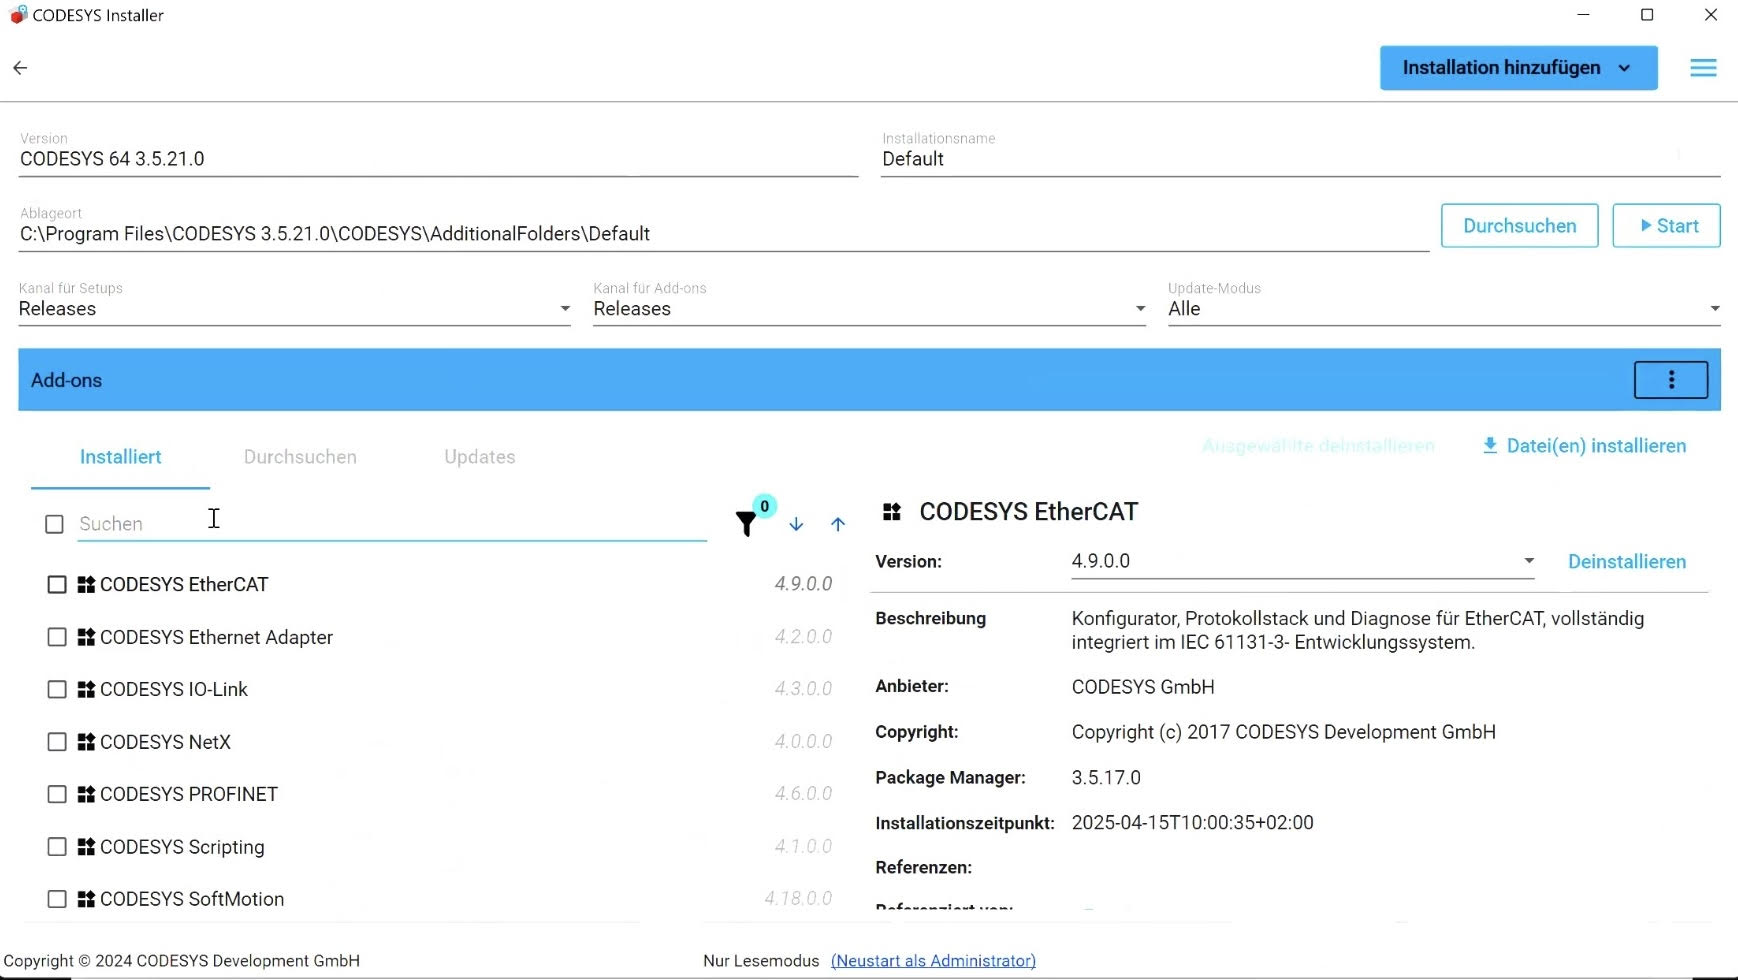
\includegraphics[width=1\textwidth]{1.jpg}
	\caption{Overview of CODESYS package Manager. Search for the following Packages in the Search Bar}
	\label{fig:packages-overview}
\end{figure}

\begin{itemize}
	\item \textbf{CODESYS Control for Linux SL} \\
	\textit{Note: ARM devices are currently not supported.}
	\item \textbf{CODESYS Control SL Deploy Tool}
	\item \textbf{CODESYS Edge Gateway for Linux SL}
\end{itemize}



\subsection{For Running Multiple Controllers with a Container Engine (e.g. Docker)}
When running multiple SoftSPS instances on the same host:
\begin{itemize}
	\item \textbf{CODESYS Virtual Control for Linux SL}
	\item \textbf{CODESYS Virtual Safe Control SL}
\end{itemize}

\subsection{For Safety Features with CODESYS}
If safety-relevant controllers are to be used, you additionally need:
\begin{itemize}
	\item \textbf{CODESYS Safety Extension}
	\item \textbf{CODESYS Safe Control Service} \\
	\textit{Only required for systems with Safe Control Core.}
	\item{To integrate PROFINET-based fieldbus systems: CODESYS PROFINET}
\end{itemize}

\newpage

\section{Software Requirements of the Host Device}

The host device must currently meet the following software requirements to ensure proper installation and operation of the necessary CODESYS packages.

\subsection*{Architecture and Compatibility}

\begin{itemize}
	\item The host must use a \textbf{64-bit CPU (AMD64 architecture)}.
	\item The operating system must support the \textbf{i386 (32-bit)} architecture. This is required specifically for using \texttt{CODESYS Control for Linux SL - AMD64} in combination with \texttt{Safe Control}, which requires 32-bit support.
	\item To enable 32-bit support on Debian-based systems, execute the following commands:
\end{itemize}

\begin{lstlisting}
sudo dpkg --add-architecture i386
sudo apt update
sudo apt install libc6-i386
\end{lstlisting}

\subsection*{Operating System Requirements}

\begin{itemize}
	\item The host device should run a \textbf{Debian-based distribution} that supports the \texttt{dpkg} package manager.
	\item RPM-based systems (e.g., Red Hat) can be used as well. As of version \textbf{4.15.0.0}, the Linux Deploy Tool supports manual installation of RPM packages.
\end{itemize}

\subsection*{Real-Time Capability}

\begin{itemize}
	\item The Linux system must provide \textbf{real-time capability}.
	\item For optimal configuration and tuning of the real-time environment, please refer to the official CODESYS online documentation:
	
	\url{https://content.helpmecodesys.com/de/CODESYS%20Control/_rtsl_performance_optimization_linux.html}
\end{itemize}

\newpage
\section{Network Configuration}

For stable operation and correct communication with CODESYS and the Timeprovider, the following network configuration is recommended:

\begin{figure}[H]
	\centering
	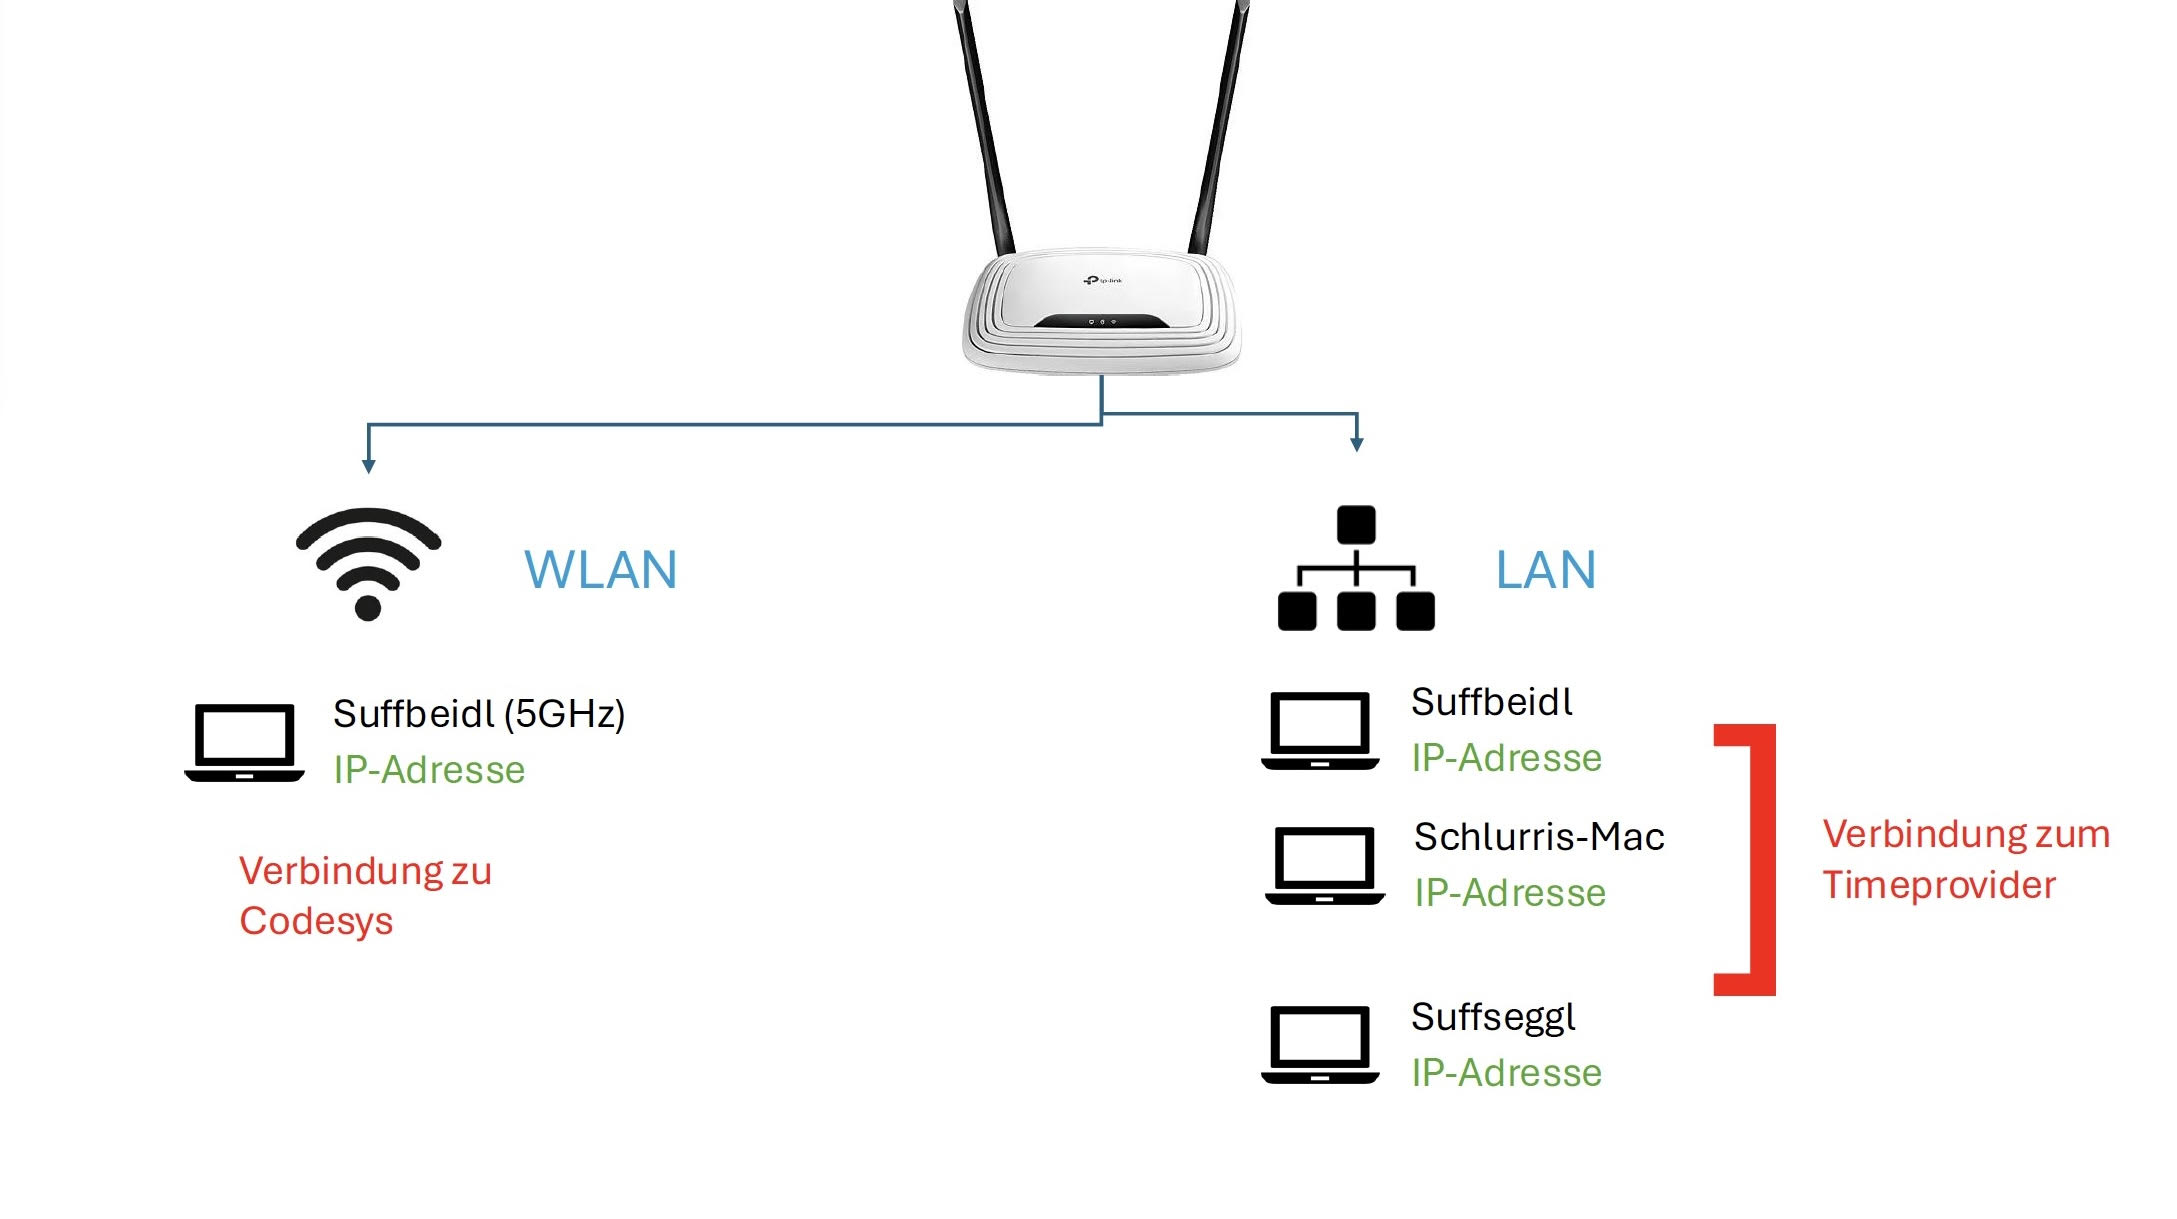
\includegraphics[width=1\textwidth]{2.jpg}
	\caption{Recommended network configuration with WLAN and LAN devices}
\end{figure}

\subsection*{Network Structure}

The network consists of a central router that provides both WLAN and wired LAN connections. The individual devices in the network are connected as follows:

\begin{itemize}
	\item \textbf{WLAN:}
	\begin{itemize}
		\item A Windows PC with CODESYS is connected via WLAN.
		\item This device has an assigned IP address and establishes the connection to the CODESYS controller.
	\end{itemize}
	
	\item \textbf{LAN:}
	\begin{itemize}
		\item All LAN devices also have static IP addresses.
		\item These devices are connected via LAN to a \textbf{Timeprovider} to provide a precise time source within the network.
	\end{itemize}
\end{itemize}

Two dedicated systems are required to ensure certification and thus security.

\newpage
\section{Installing Runtime Systems}


With the CODESYS Deploy Tool, a connection can be established to the Linux host where the necessary package-based or container-based runtime systems are to be installed.  
Navigate to:  
\texttt{Tools → Deploy Control SL → Connect to the Linux target system via SSH connection.}


In the \textbf{Deployment} tab, all available package- and container-based runtime system versions and components that can be installed on the device are listed.  
Here, the appropriate package (or container) and its version can be selected and installed on the Linux device.

\begin{figure}[H]
	\centering
	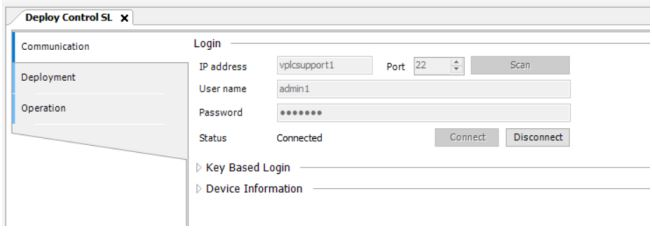
\includegraphics[width=1\textwidth]{3.jpg}
	\caption{Open Deploy Control: shows target device's IP address (WLAN), username ("with root access"), and Linux user password input}
\end{figure}


\section{Deployment to use Control Linux SL (without Docker)}

For the usage of CODESYS Control for Linux SL you have to install the following Packages:

\begin{figure}[H]
	\centering
	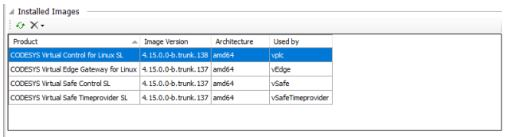
\includegraphics[width=1\textwidth]{4.jpg}
	\caption{What you see under "Deployment"}
\end{figure}
\newpage


\section{Installing CODESYS Virtual Control for Linux SL}

This section provides a comprehensive guide for deploying the CODESYS Virtual Control for Linux SL runtime environment, including both a virtual standard PLC (vPLC) and a virtual safety PLC (vSafePLC) with a dedicated Timeprovider. The deployment is split across two separate Linux systems for real-time safety certification and architectural integrity.

\subsection{Deployment Overview (Using Docker Containers)}

To implement this scenario, the following setup is required:

\begin{itemize}
	\item \textbf{Linux Host PC 1} – Hosts the vPLC and vSafePLC runtime systems.
	\item \textbf{Linux Host PC 2} – Hosts the Safety Timeprovider service.
\end{itemize}

An internet connection and Docker must be available on both systems. SSH should be configured to allow remote connection via the CODESYS Deploy Tool.

\vspace{0.5em}
Refer to the official CODESYS documentation for background:
\url{https://content.helpme-codesys.com/en/CODESYS%20Control/_rtsl_scenario_safe_house.html}

\subsection*{Step 1: Install the vSafe Timeprovider on Linux Host PC 2}

\begin{enumerate}
	\item Launch the CODESYS Deploy Tool.
	\item Connect to \textbf{Linux Host PC 2} via \texttt{Tools → Deploy Control SL → Communication tab}.
	\item Switch to the \textbf{Deployment} tab.
	\item Select \texttt{CODESYS Virtual Safe Time Provider SL} from the product list.
	\item Choose the latest available version and click \texttt{Install}.
	\item Switch to the \textbf{Operation} tab and click the \texttt{+} button to add a new instance.
	\item Name the instance \texttt{timeprovider}, select \textbf{Safety Timeprovider} from the filter list, and use the latest version.
	\item In the instance settings:
	\begin{itemize}
		\item Set \texttt{TARGET\_IP} to the IP address of \textbf{Linux Host PC 1}.
		\item Ensure \texttt{TARGET\_PORT} is \texttt{60000}.
		\item Set \texttt{Autostart} to \texttt{Yes}.
	\end{itemize}
	\item Click \texttt{Save}, then \texttt{Start} the instance.
\end{enumerate}

\begin{figure}[H]
	\centering
	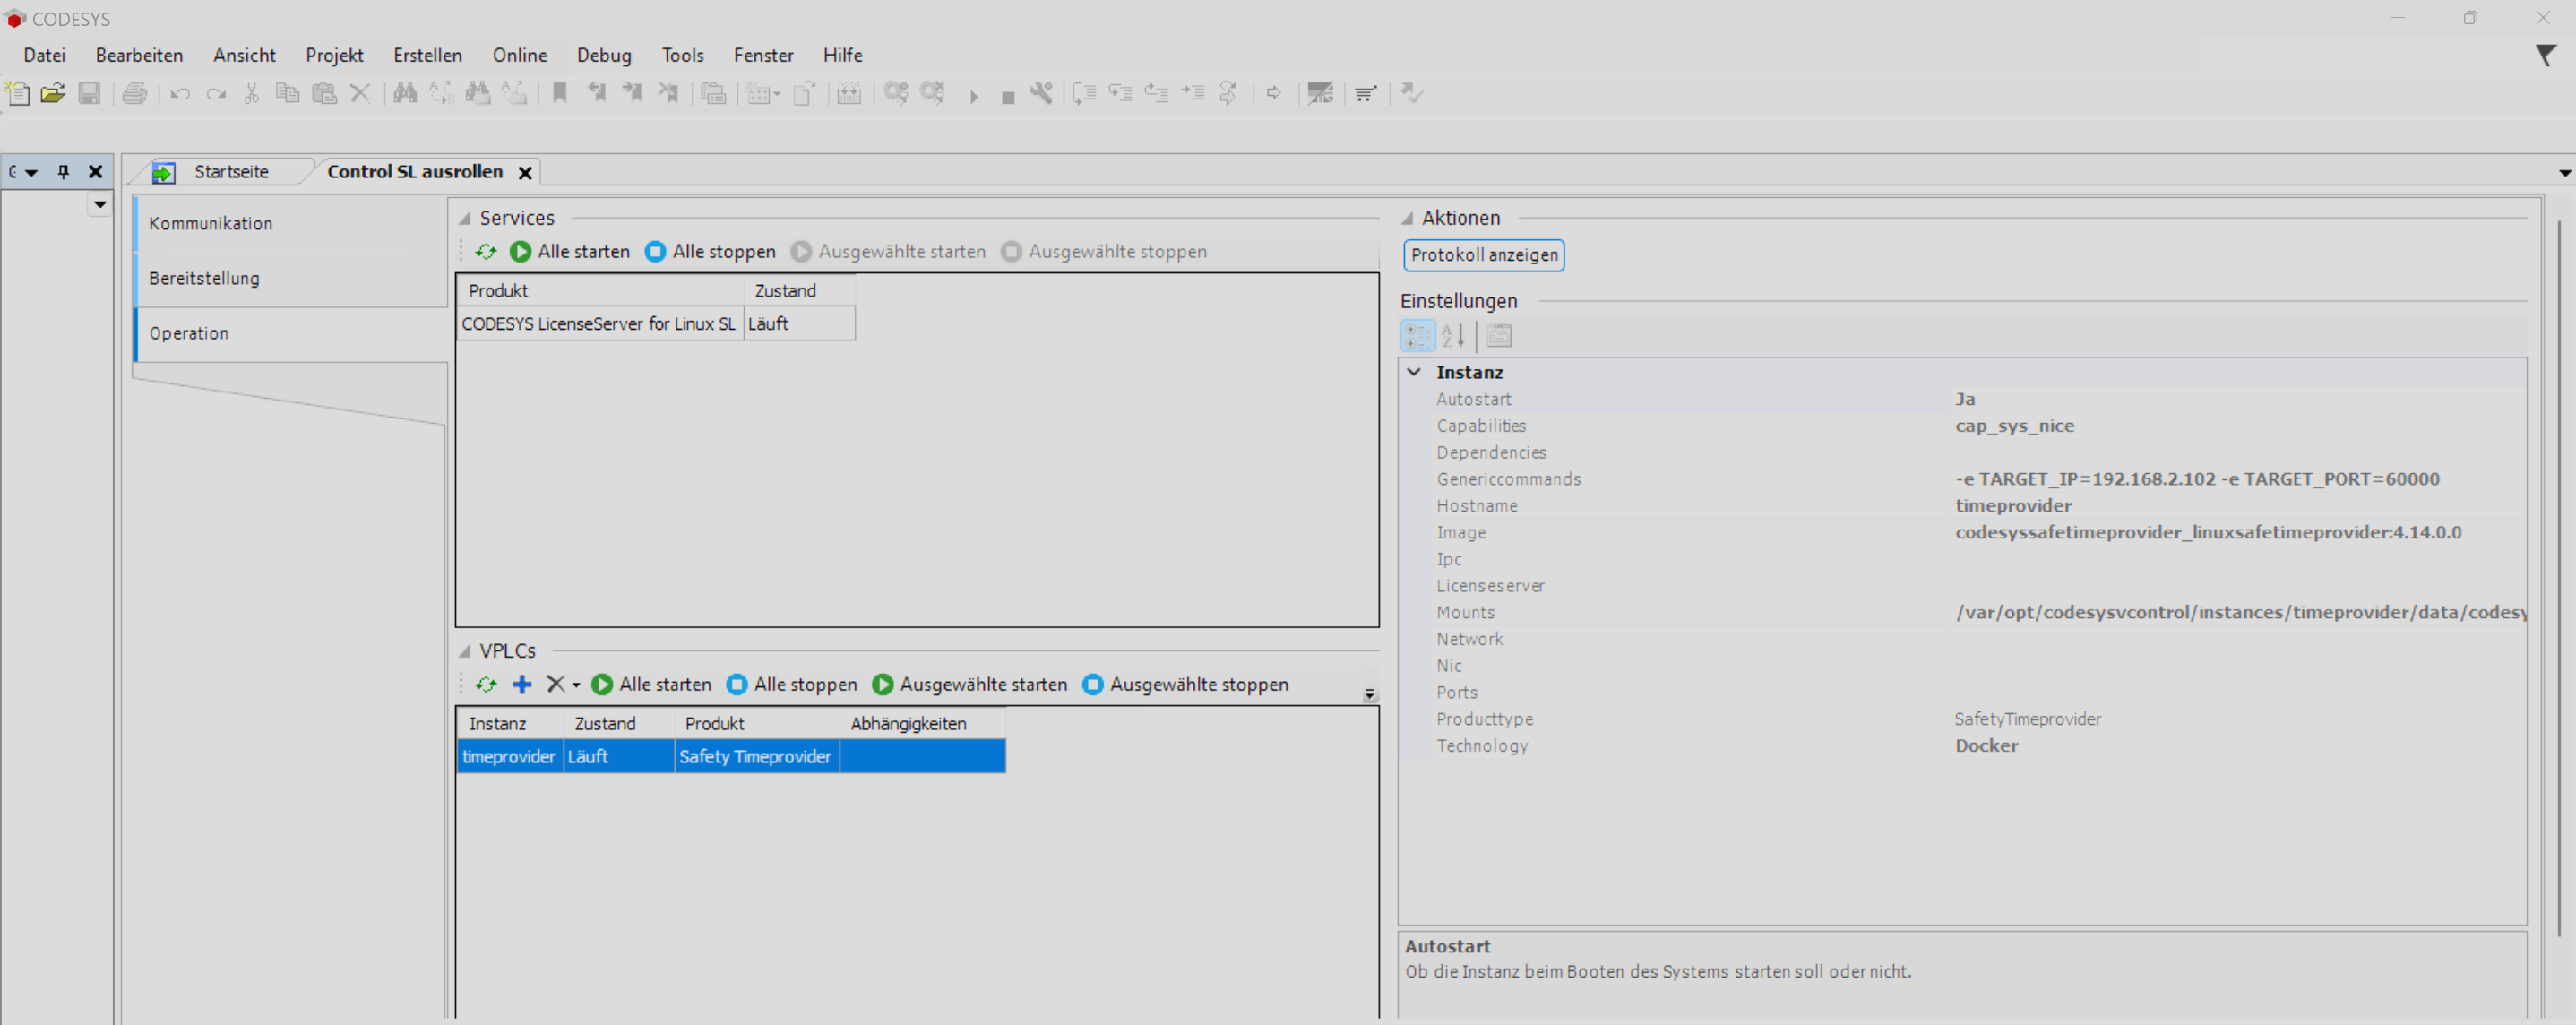
\includegraphics[width=1\textwidth]{5.PNG}
	\caption{Deploy Tool – Configuration of Timeprovider instance on Linux Host PC 2.}
\end{figure}

\subsection*{Step 2: Install vPLC and vSafePLC on Linux Host PC 1}

\begin{enumerate}
	\item Connect to \textbf{Linux Host PC 1} via the CODESYS Deploy Tool.
	\item In the \textbf{Deployment} tab, install:
	\begin{itemize}
		\item \texttt{CODESYS Virtual Control SL} (vPLC)
		\item \texttt{CODESYS Virtual Safe Control SL} (vSafePLC)
	\end{itemize}
	\item Go to the \textbf{Operation} tab and click \texttt{+} to add new instances:
	\begin{itemize}
		\item Create \texttt{vPLC} – Select \textbf{Runtime System}.
		\item Create \texttt{vSafePLC} – Select \textbf{Safety Runtime System}.
	\end{itemize}
	\item Configure the \texttt{vSafePLC} instance:
	\begin{itemize}
		\item \texttt{Ports}: \texttt{60000:60000/udp}
		\item \texttt{IPC}: \texttt{container:vPLC}
		\item \texttt{Dependencies}: \texttt{vPLC} must start first
	\end{itemize}
	\item Configure the \texttt{vPLC} instance:
	\begin{itemize}
		\item Enable \texttt{shareable} IPC namespace
	\end{itemize}
	\item Click \texttt{Start All} to run both instances.
\end{enumerate}

\begin{figure}[H]
	\centering
	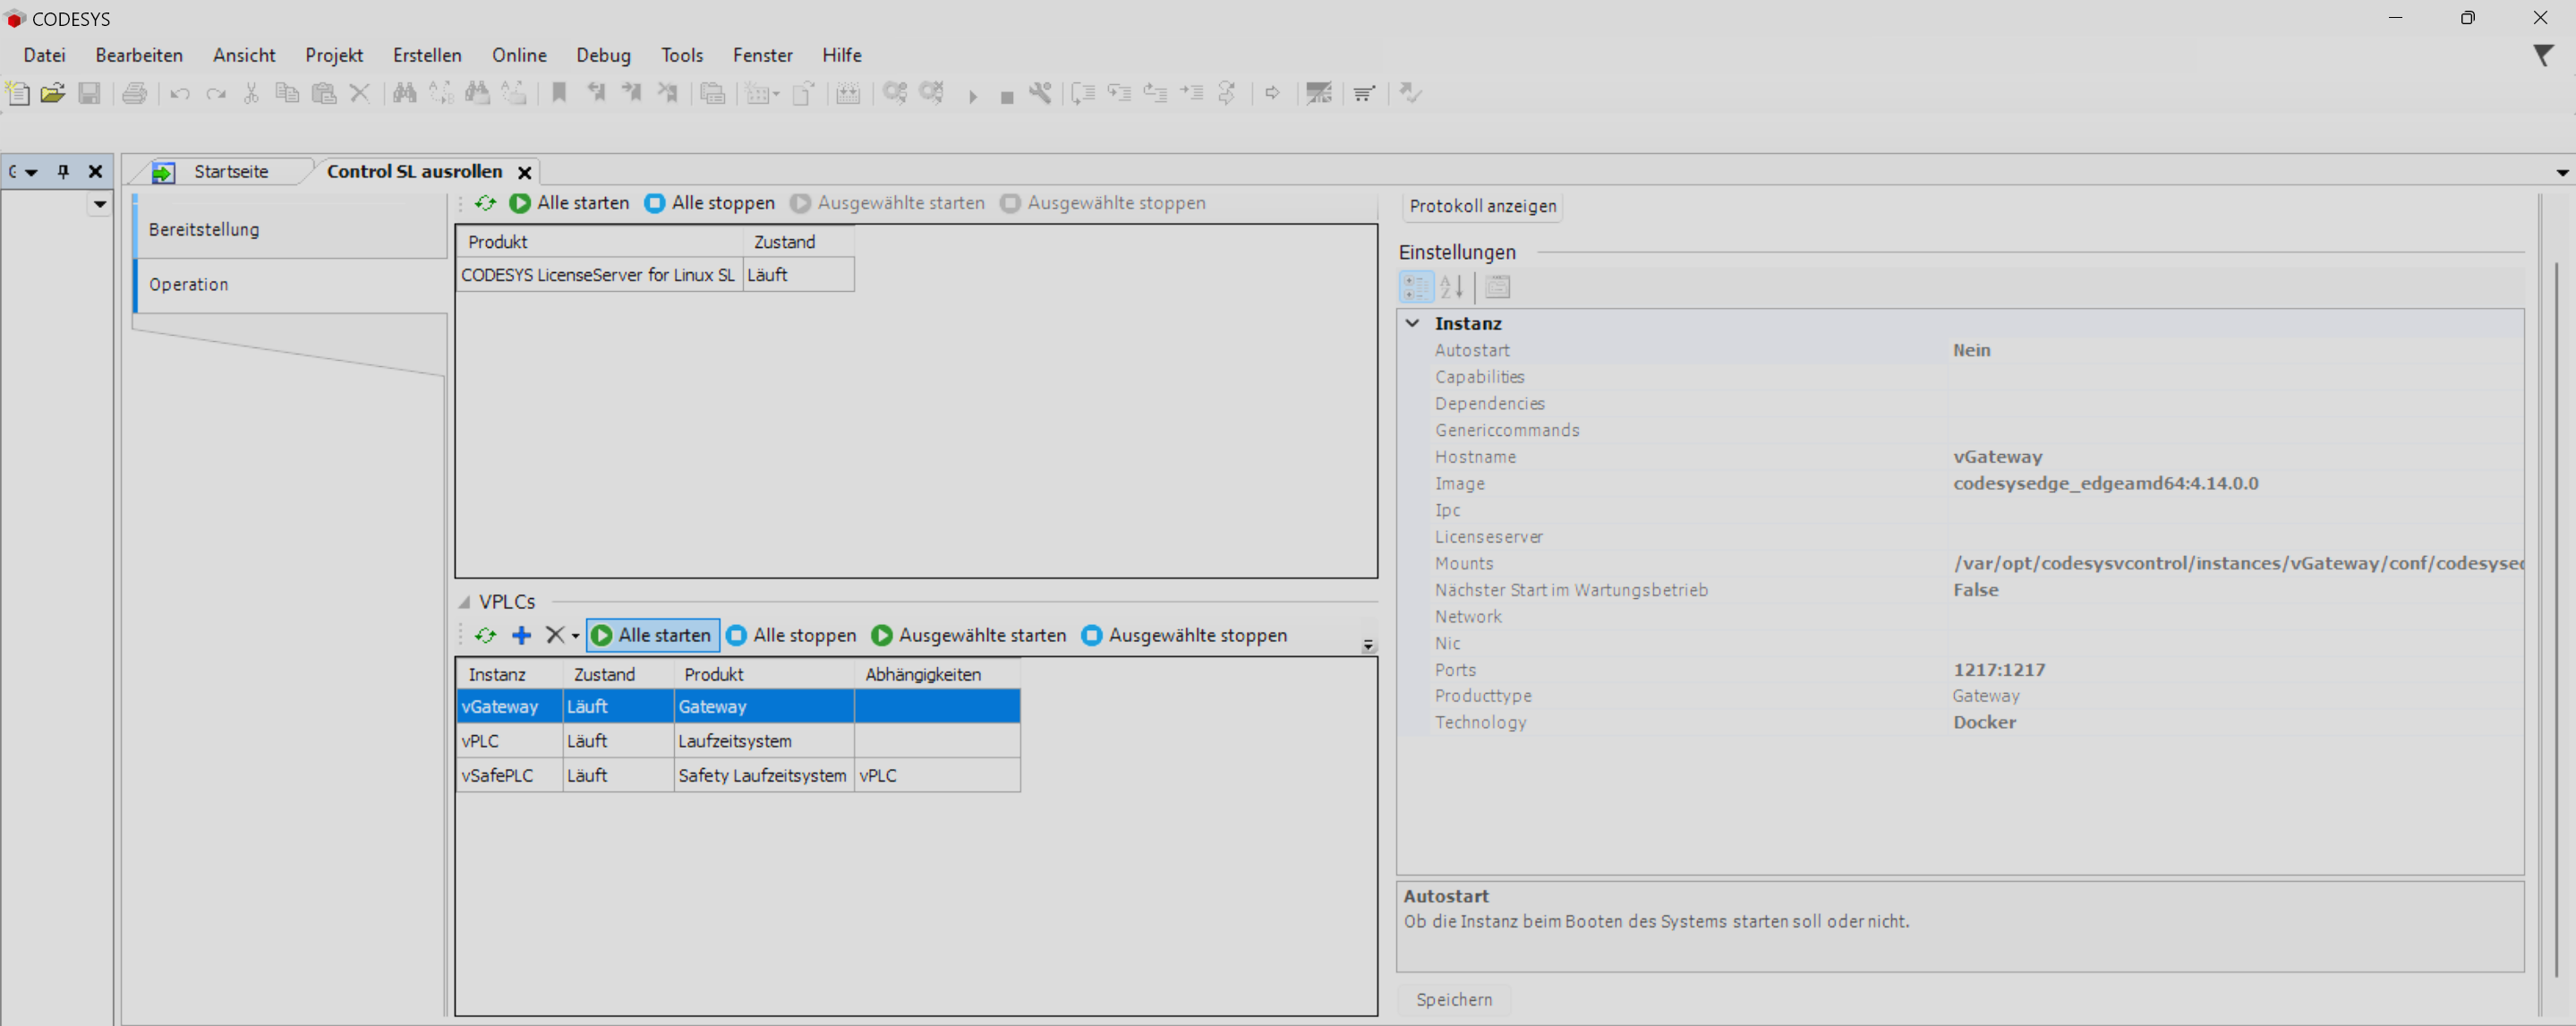
\includegraphics[width=1\textwidth]{6.PNG}
	\caption{VGateway Configurations. Feel free to copy the Mounts}
\end{figure}

\begin{figure}[H]
	\centering
	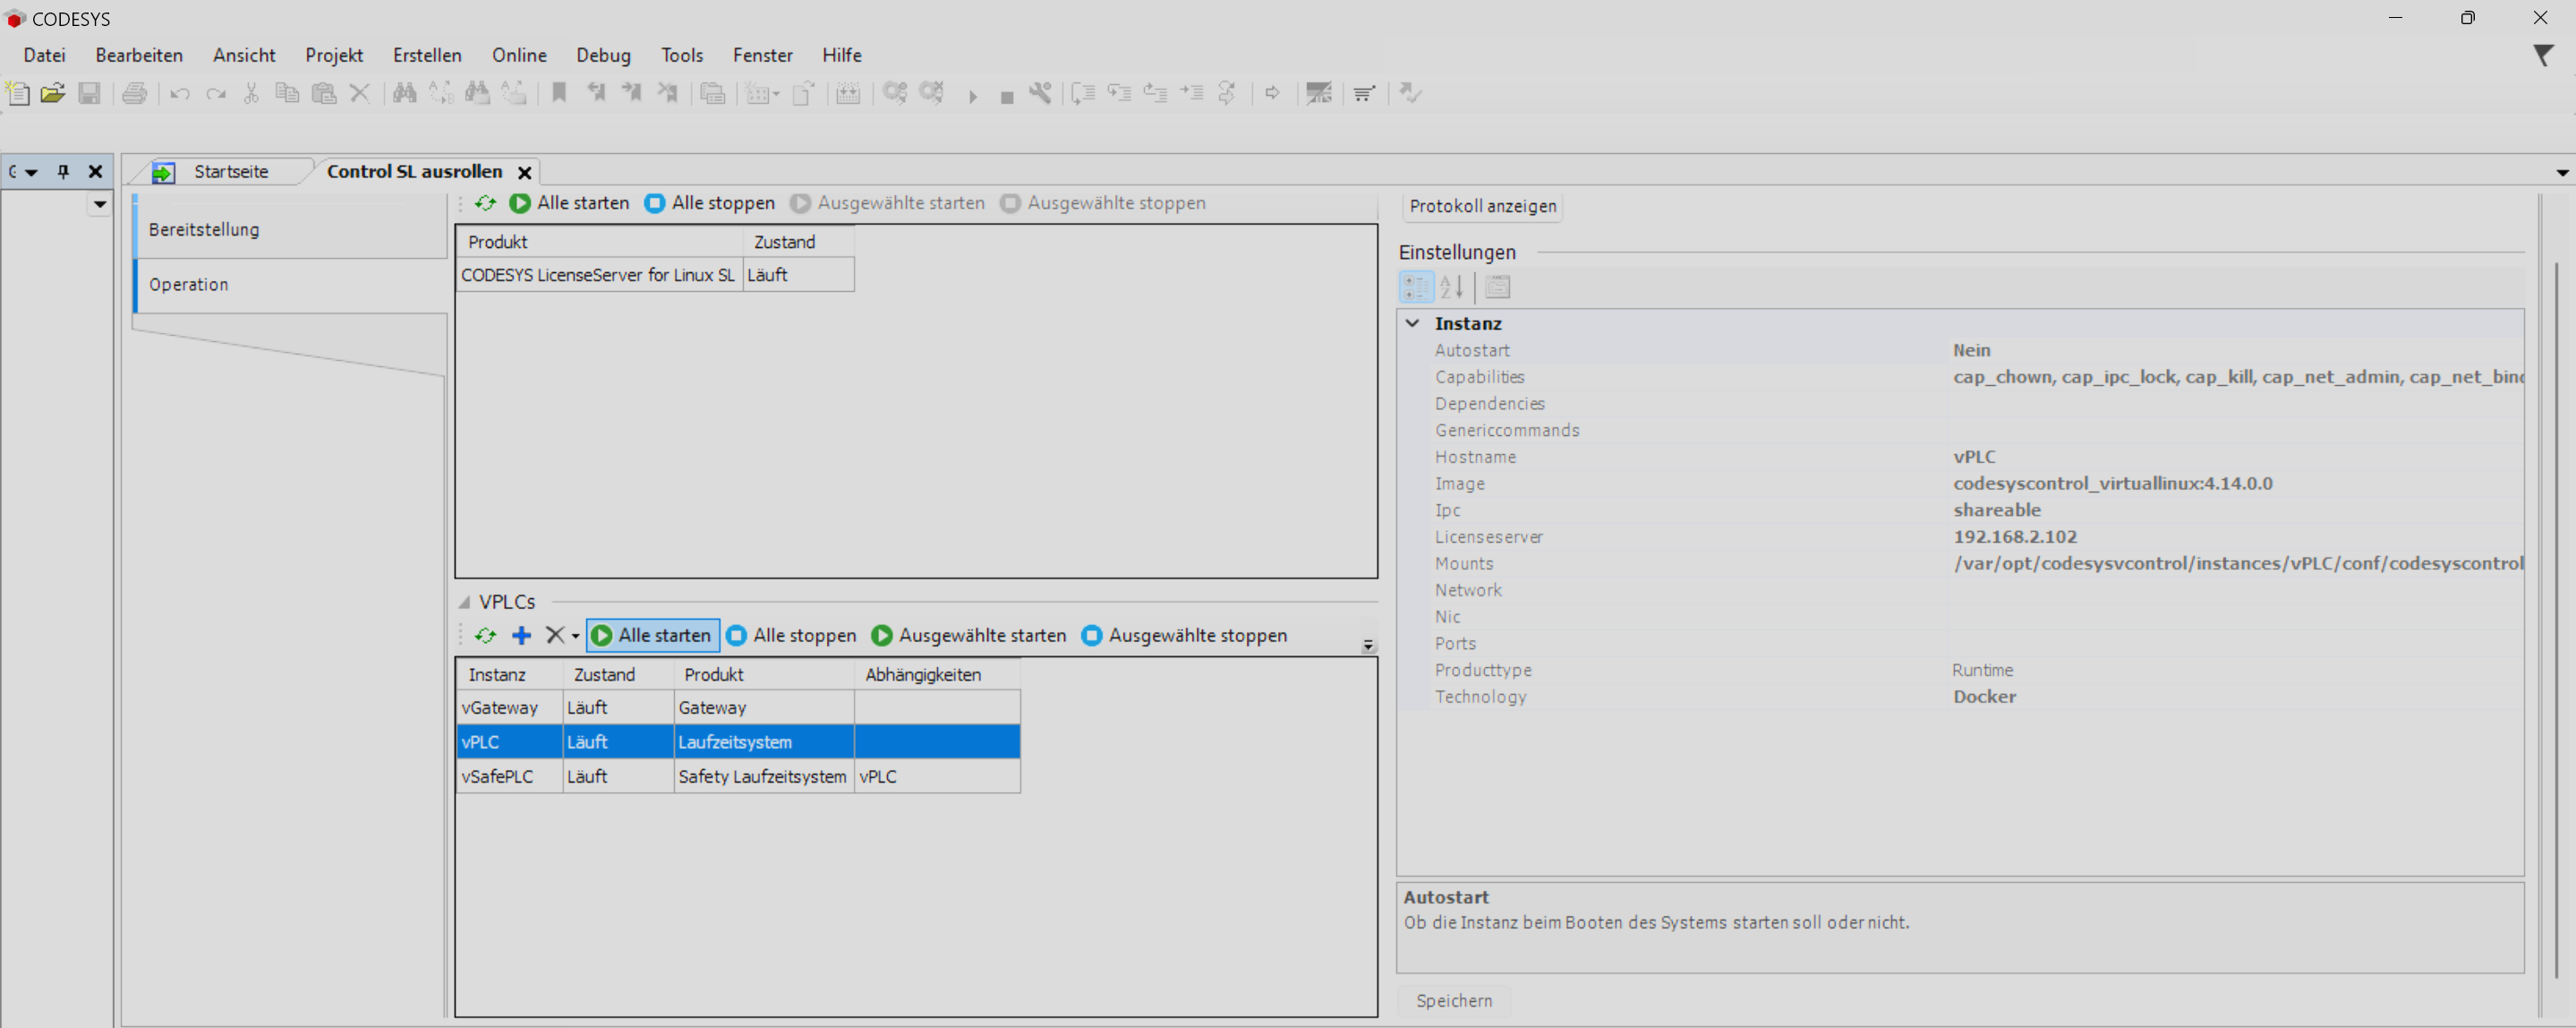
\includegraphics[width=1\textwidth]{7.PNG}
	\caption{VPLC Configurations}
\end{figure}

\begin{figure}[H]
	\centering
	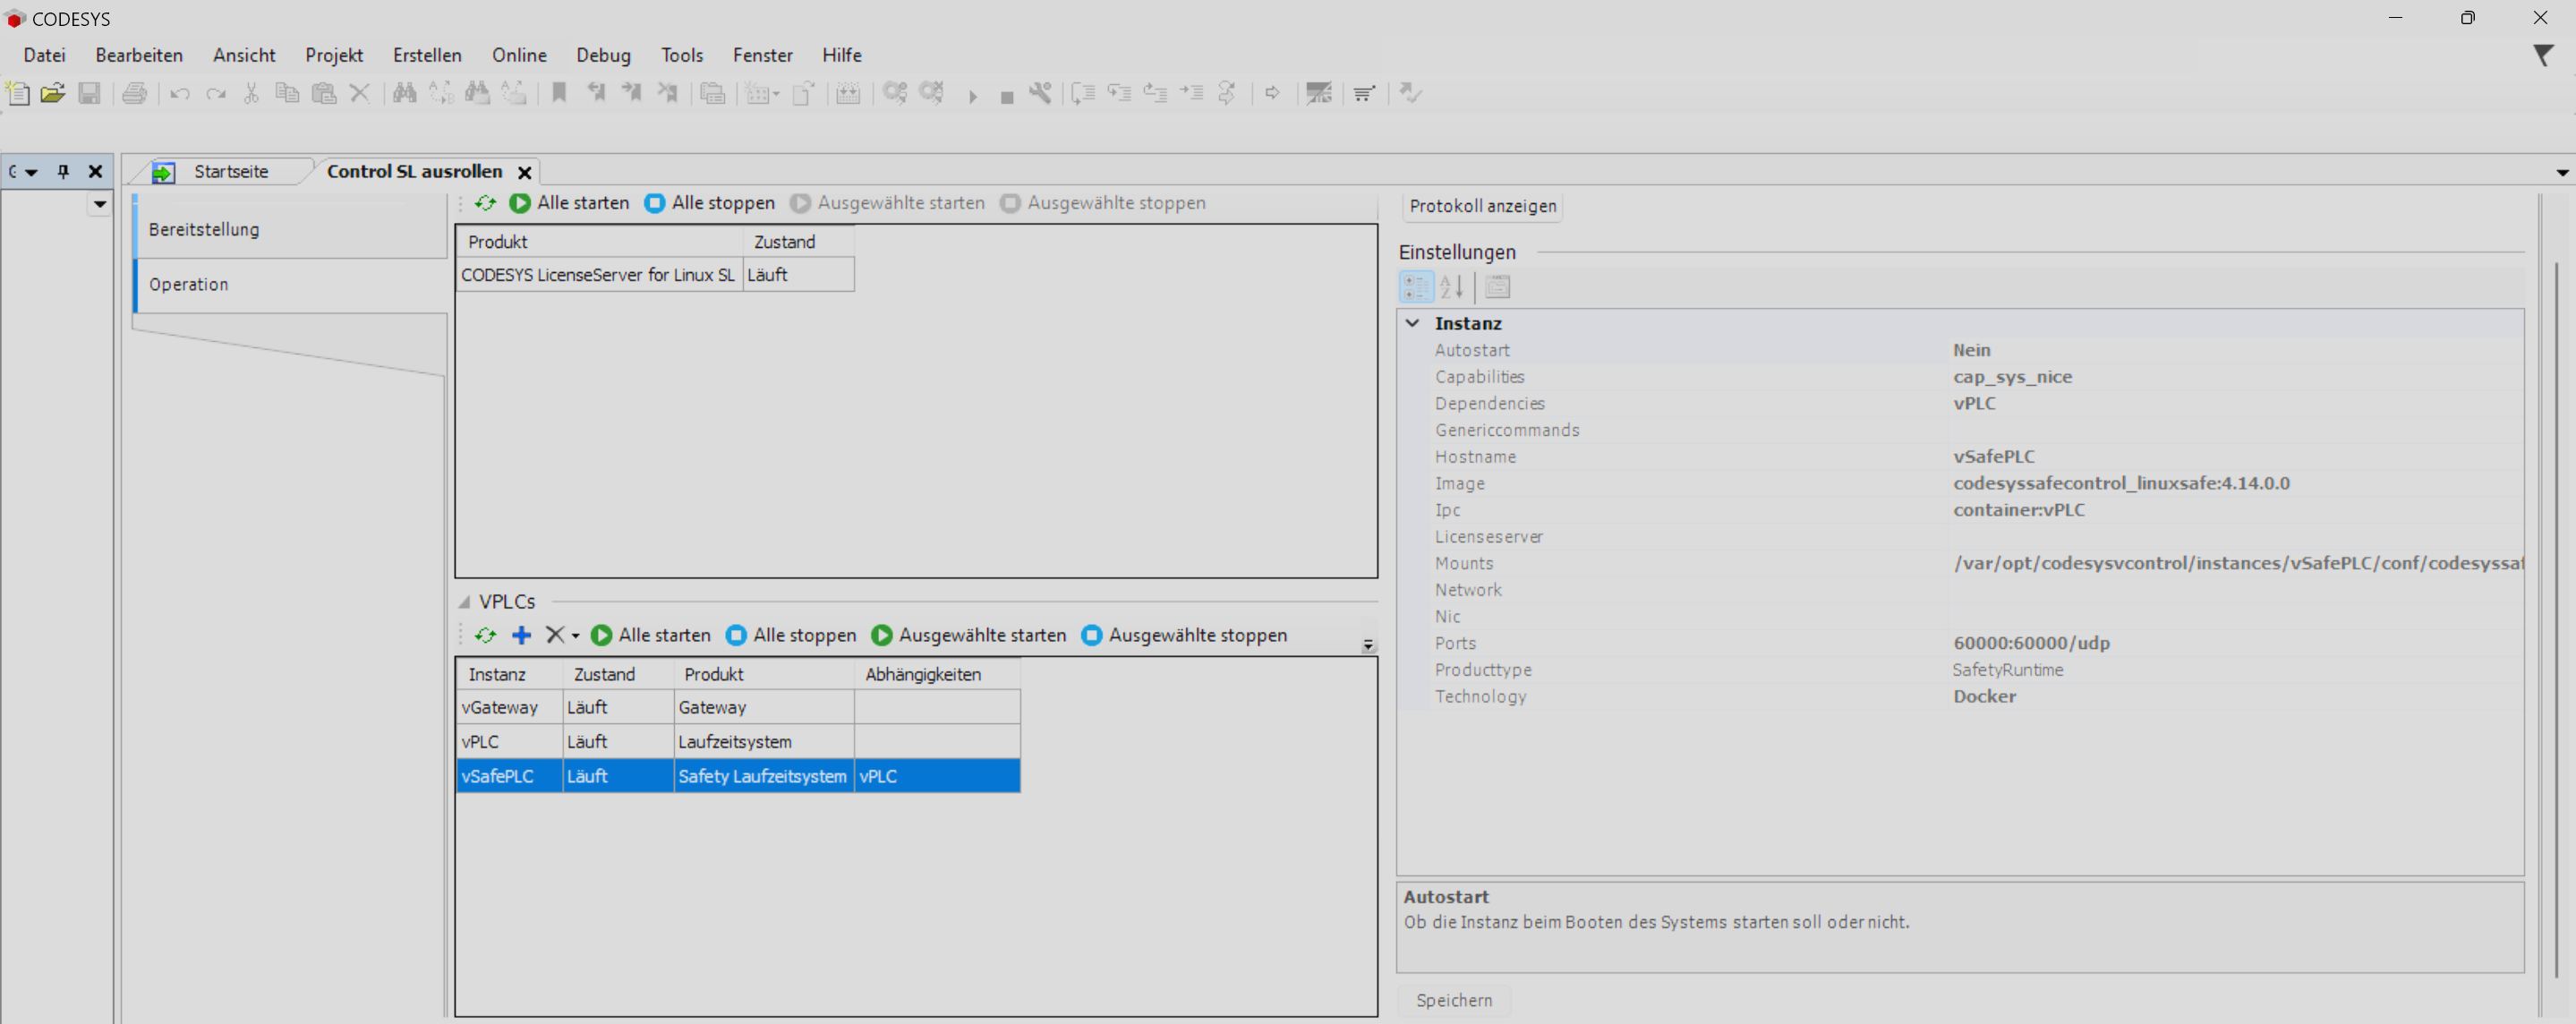
\includegraphics[width=1\textwidth]{8.PNG}
	\caption{Use the same Mounts}
\end{figure}

\subsection*{Step 3: Verify the Time Synchronization}

To confirm proper communication between the Timeprovider and vSafePLC:

\begin{itemize}
	\item In the Deploy Tool, select the \texttt{vSafePLC} instance.
	\item Open the log via the \texttt{Show Log} action in the top-right corner.
	\item Check for the message: \texttt{External Time Provider found}.
\end{itemize}

If this message is present, the safety time synchronization is functioning correctly.

\vspace{0.5em}
All runtime systems are now installed and running. You can proceed to create your project and integrate PROFIsafe.

\newpage


\section{CODESYS Project for Using CODESYS Safe Control}
\label{sec:safe_control_project}

\subsection{Importing Devices}
To automatically generate the logical safety devices in the device tree, a specific import option must be enabled in the PROFINET plugin.

After enabling this setting, re-import the GSDML file for the corresponding PROFINET fieldbus devices.

\begin{figure}[H]
	\centering
	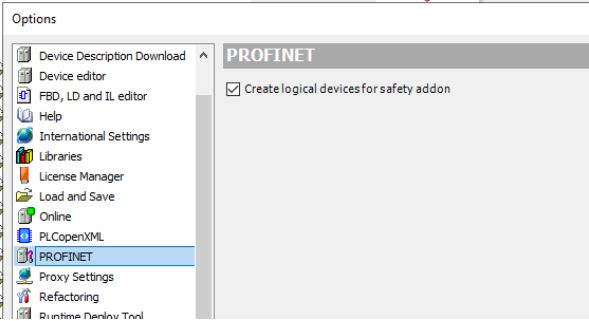
\includegraphics[width=0.8\textwidth]{9.JPG}
	\caption{VPLC Configurations}
\end{figure}

\textbf{Note:} Ensure the following option is enabled: \\
\texttt{Options → PROFINET → Create logical devices for safety addon}

\subsection{Creating a New Project}
\textbf{Note:} Using the \textit{Empty Safety Project} template will automatically enable user management for the safety project.

Alternatively, you can use the \textit{Empty Project} or \textit{Standard Project} templates.  
If using the \textit{Standard Project}, select the following device:  
\texttt{CODESYS Control for Linux SL (CODESYS)}

\begin{figure}[H]
	\centering
	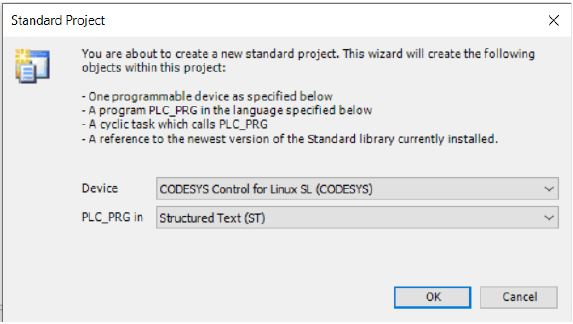
\includegraphics[width=0.8\textwidth]{10.JPG}
\end{figure}

In the project tree, right-click on the device and select:  
\texttt{Add Device → PLCs},  
then choose the appropriate \texttt{CODESYS Safe Control} device to add it to your project.

\begin{figure}[H]
	\centering
	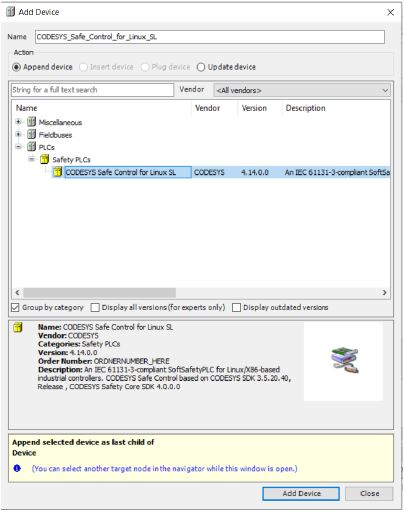
\includegraphics[width=0.6\textwidth]{11.JPG}
\end{figure}

\subsection{Project Tree Overview}
After adding the \texttt{CODESYS Safe Control for Linux SL} controller, the project tree now includes:

\begin{itemize}
	\item A dedicated \textbf{Safety Logic}
	\item A \textbf{Safety Application}
	\item A separate \textbf{Library Manager}
	\item Logical \textbf{I/Os}
	\item A defined \textbf{Safety Task}
\end{itemize}

\begin{figure}[H]
	\centering
	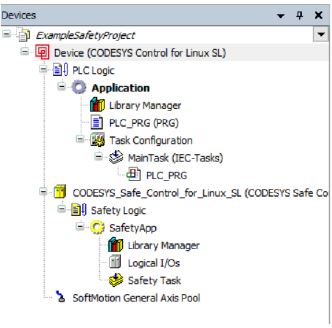
\includegraphics[width=0.5\textwidth]{12.JPG}
\end{figure}

These components provide the foundation for developing and managing the safety-related aspects of your application in CODESYS.

\subsection{Communication with Linux Runtime Systems}

To establish communication between the CODESYS development environment and the Linux runtime system, a gateway is required. This can either be a local gateway or a \textbf{CODESYS Edge Gateway for Linux} installed directly on the target device.

\begin{figure}[H]
	\centering
	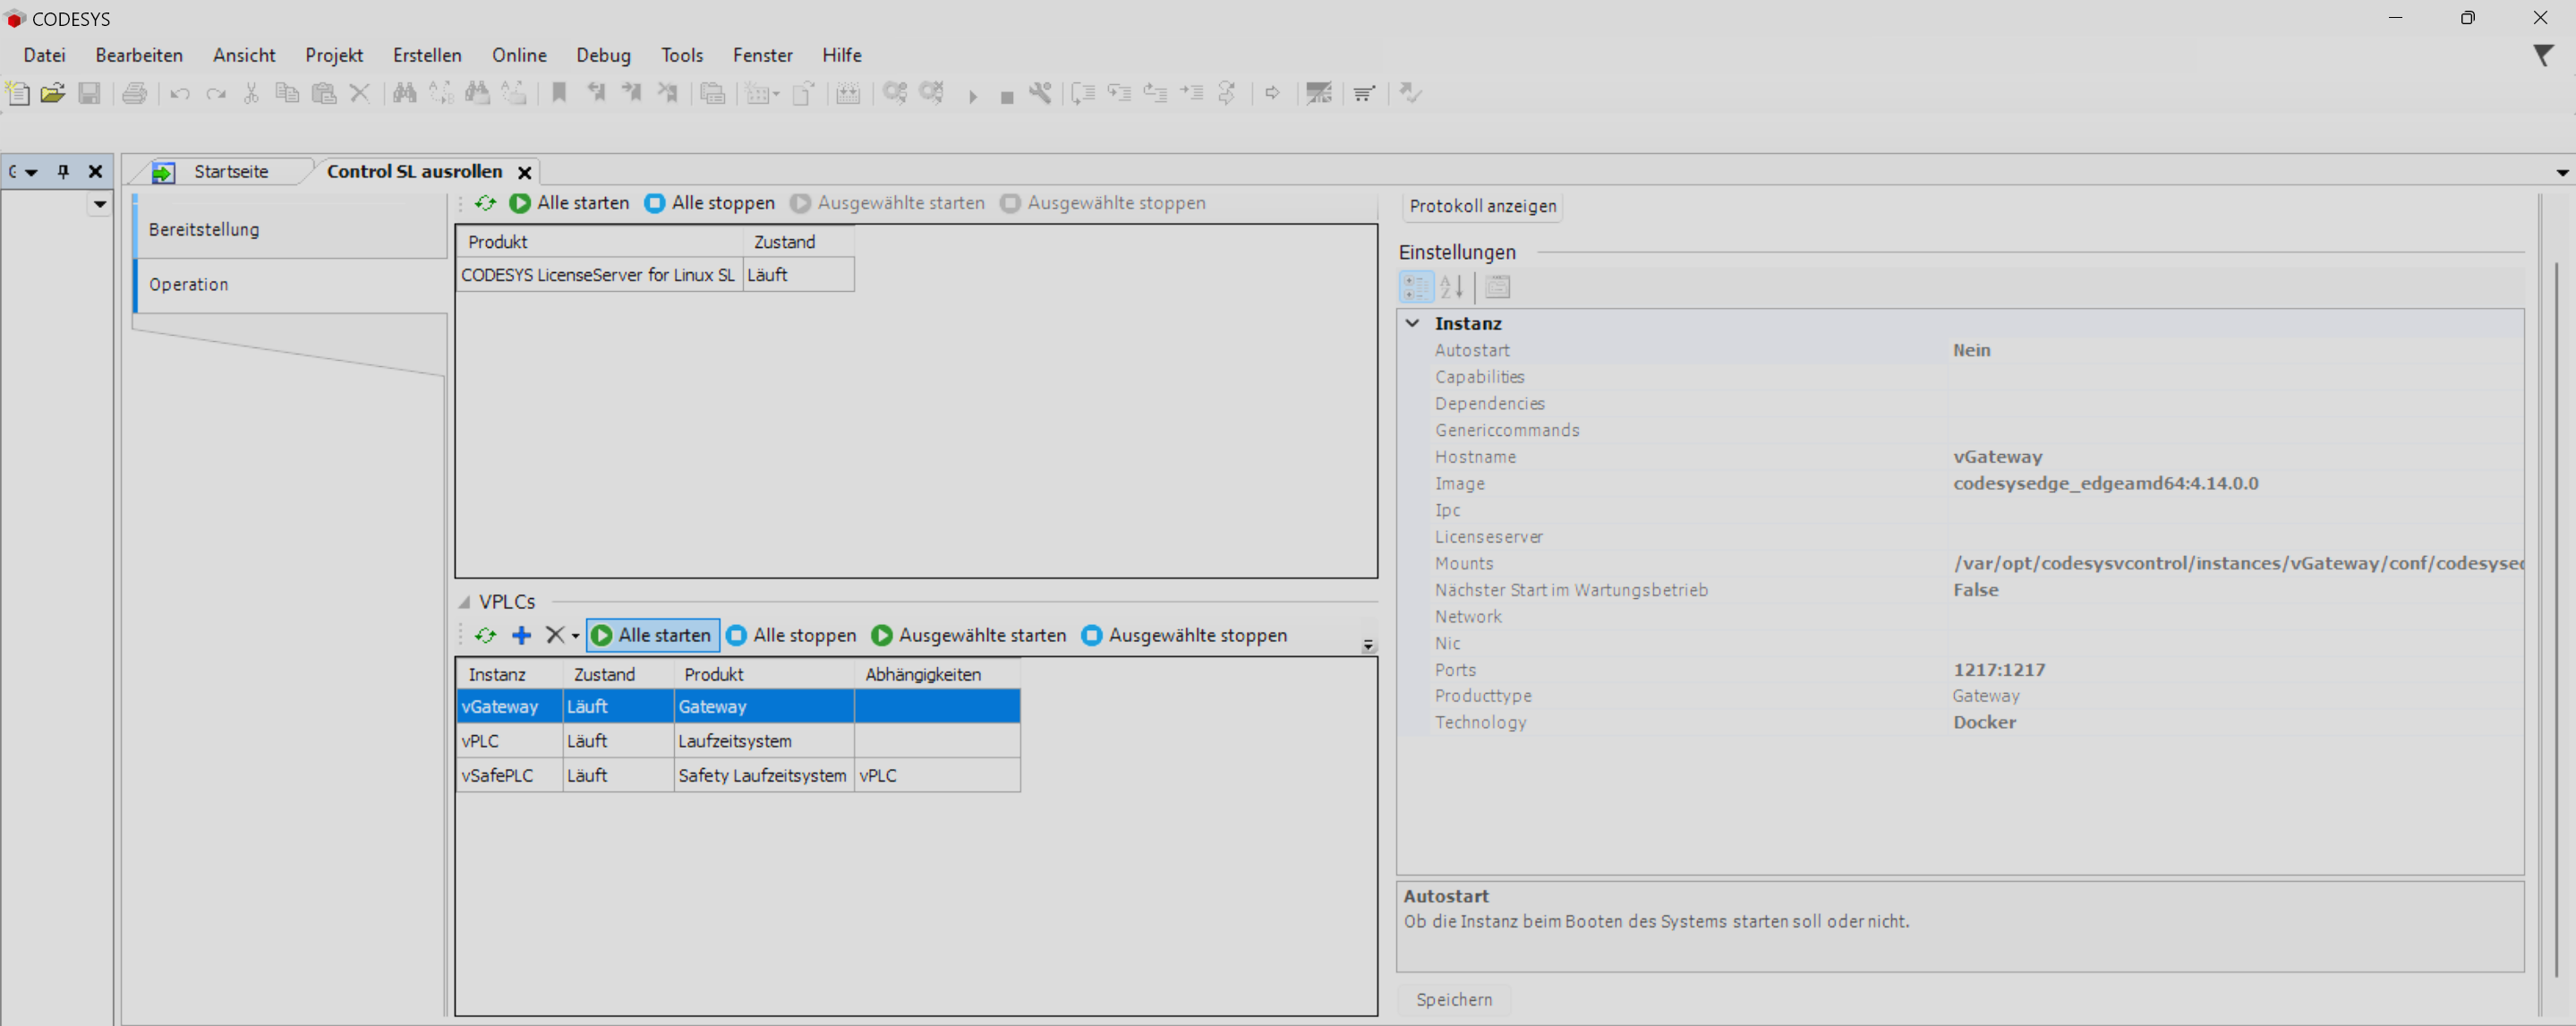
\includegraphics[width=1\textwidth]{gateway.png}
\end{figure}

Initial setup instructions for installing the gateway and establishing communication with a Linux runtime can be found here:

\begin{quote}
	\url{https://content.helpme-codesys.com/en/CODESYS%20Control/_rtsl_load_and_start_application.html}
\end{quote}

\subsection{Installing a Safe Timeprovider}

A \textbf{Safe Timeprovider} is always required for the operation of hardware-independent Safe Control runtime systems. This component is available as a separate software package and provides essential timing information for safety-related applications.

For improved fault detection, the timeprovider should run on a \textbf{second device} with a different CPU. It periodically sends a timestamp to the device running the safety controller, allowing it to compare and detect discrepancies in CPU clock timing—an important aspect of safety certification.

\vspace{0.5em}
\textbf{Development and Testing:}  
For initial testing, offline programming, or virtual commissioning, the timeprovider may also be installed on the \textbf{same device} as the safety controller.

\vspace{0.5em}
\textbf{Production Systems:}  
For deployment in a certified application, the timeprovider \textbf{must be installed on separate hardware} to ensure safety integrity.

\vspace{0.5em}
If you are using a package-based controller, the \texttt{Safe Timeprovider SL} can be deployed via the \textbf{CODESYS Deploy Tool}.

\paragraph{Same-Device Configuration:}  
If the Safe Timeprovider runs on the same machine as the \texttt{CODESYS Safe Control}, no additional environment variable is required. The time signal is sent by default to:

\begin{itemize}
	\item \texttt{localhost} on port \texttt{9000}
\end{itemize}


\begin{figure}[H]
\centering
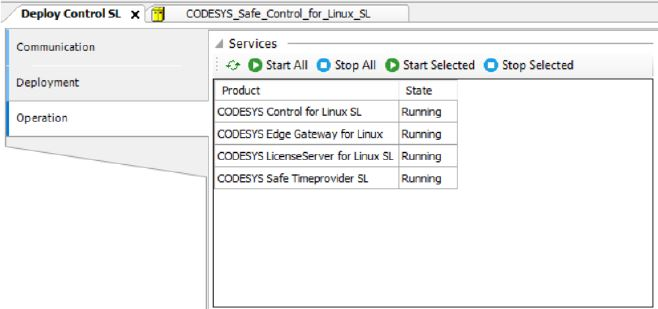
\includegraphics[width=1\textwidth]{14.JPG}
\end{figure}

\paragraph{Two-Device Configuration:}  
If the Safe Timeprovider runs on a separate Linux device, you must set the target IP address as an environment variable on that system:

\begin{lstlisting}[language=bash]
export TARGET_IP=XXXX.XXXX.XXX.XXXX
\end{lstlisting}

In the \texttt{Safe Control} log, a successful connection to the timeprovider should be visible before performing a download. This indicates that synchronization is working correctly.

\begin{figure}[H]
\centering
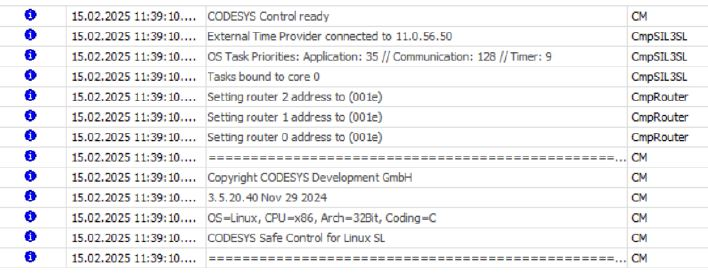
\includegraphics[width=1\textwidth]{15.JPG}
\end{figure}

\paragraph{Changing the Time Cycle:}  
The default sending cycle is \texttt{10 ms}. You can override this setting using the \texttt{CYCLETIME} environment variable. For example, to change the cycle time to \texttt{3 ms}:

\begin{lstlisting}[language=bash]
export CYCLETIME=3
\end{lstlisting}


\subsection{Example: Adding a Safe Application Program}

% Introducing the example of creating a simple counter in a safe application
As an introductory example, this section illustrates how a simple counter can be created within a safe application.

% Adding a new program using the SafetyApp context menu
By right-clicking on the \texttt{SafetyApp} and selecting \texttt{Add Object} $\rightarrow$ \texttt{Extended POU (Safety)}, a new program can be added.

\begin{figure}[H]
	\centering
	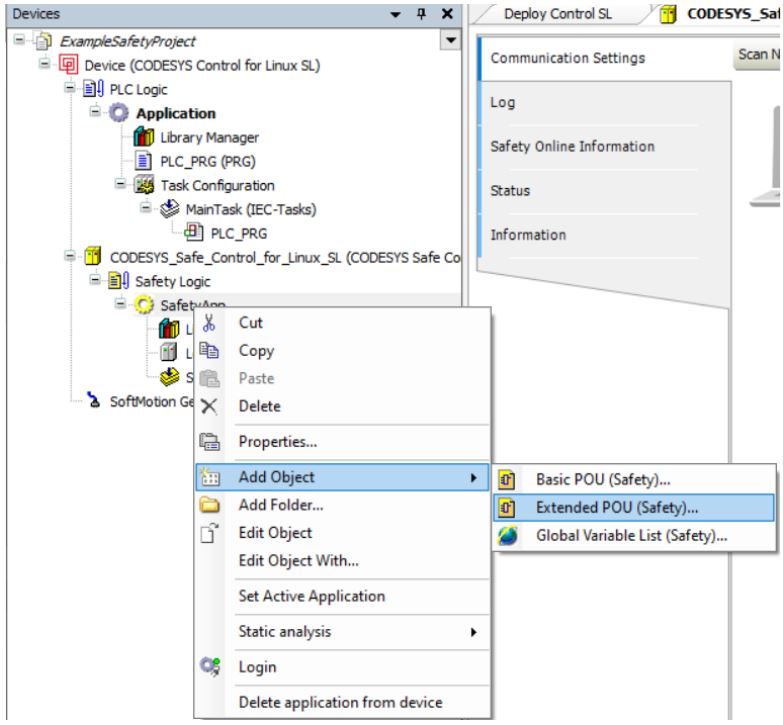
\includegraphics[width=0.5\textwidth]{e1.JPG}
\end{figure}

% Choosing between a program or function block for the POU
For the POU, a selection can be made between a program or a function block.

\begin{figure}[H]
	\centering
	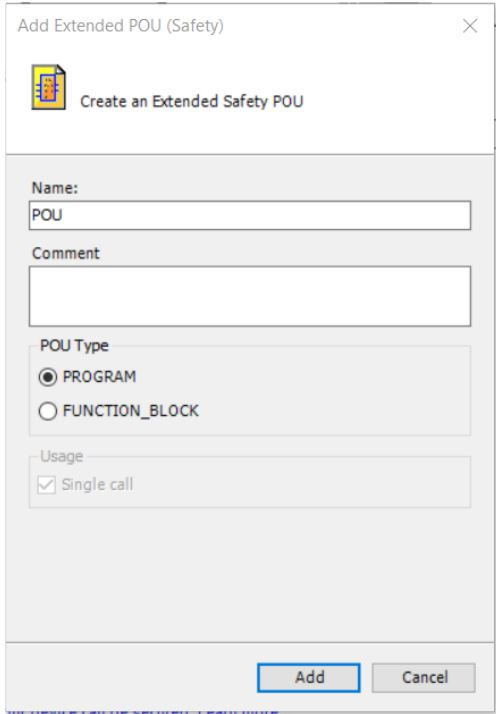
\includegraphics[width=0.4\textwidth]{e2.JPG}
\end{figure}

% Adding a network and an adder block
Within the program, a network is already defined. Using the toolbox, an \texttt{ADD} adder block with two inputs can be added.
\begin{figure}[H]
	\centering
	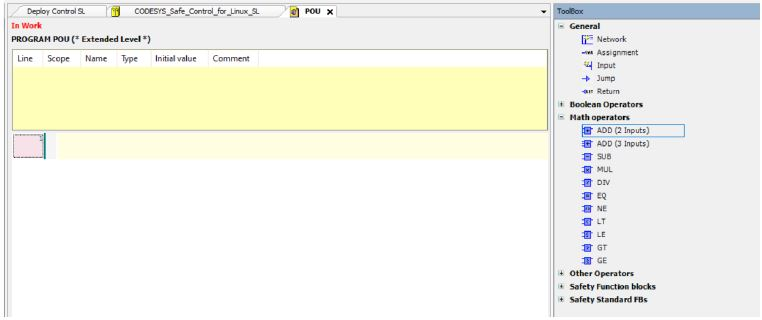
\includegraphics[width=1\textwidth]{e3.JPG}
\end{figure}
% Assigning variables to the adder block inputs
A variable named \texttt{counter} can be added to one input. The second summand can be added to the second input.
\begin{figure}[H]
	\centering
	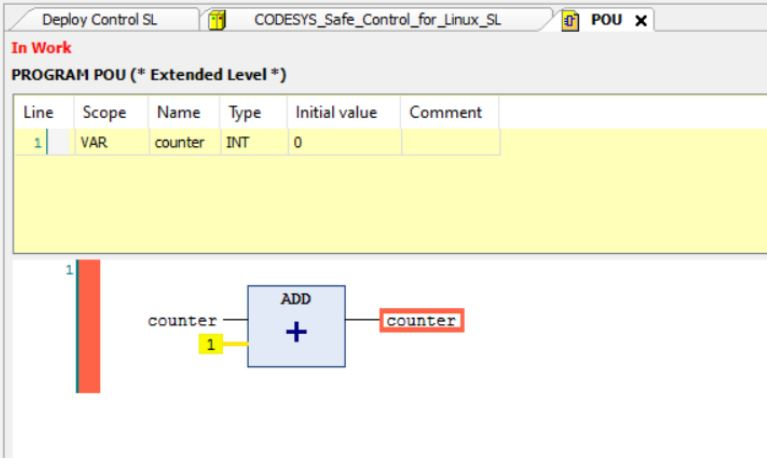
\includegraphics[width=0.8\textwidth]{e4.JPG}
\end{figure}
\label{sec:safe-pou-changes}
% Highlighting changes in a Safe POU
Changes in a Safe POU are marked in red, and this does not indicate an error.
% Adding and deleting a network to clear the red highlight
Finally, a network can be added and subsequently deleted, ensuring the POU is no longer marked in red.
\begin{figure}[H]
	\centering
	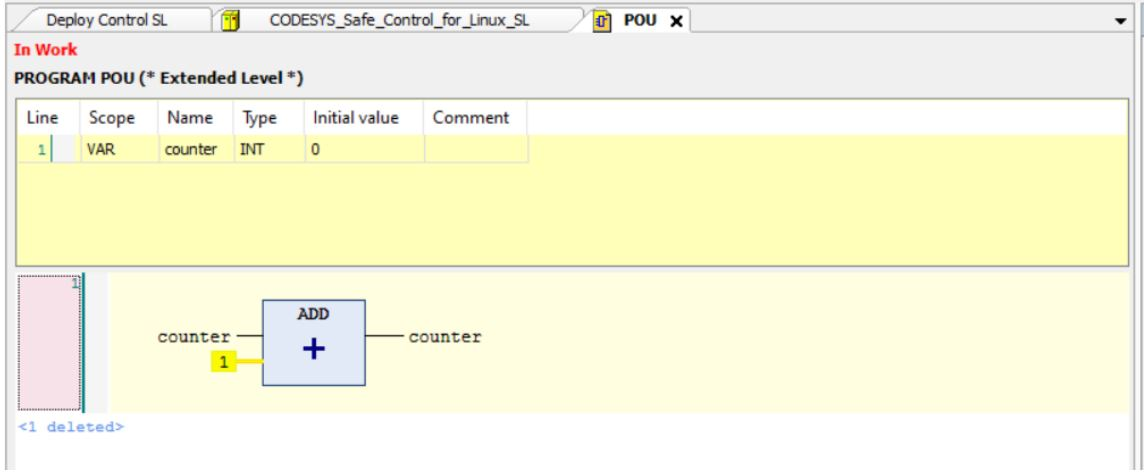
\includegraphics[width=1\textwidth]{e5.JPG}
\end{figure}
% Automatic assignment of the POU to the Safety Task
After adding the POU to the project tree, it is automatically assigned to the Safety Task.
\begin{figure}[H]
	\centering
	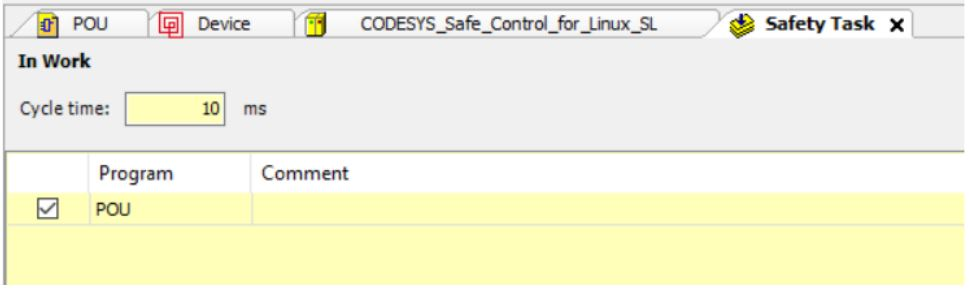
\includegraphics[width=1\textwidth]{e6.JPG}
\end{figure}
% Connecting to the Linux runtime system and downloading the project
Subsequently, you can connect to the Linux runtime system and download the project to the target device. 
\begin{figure}[H]
	\centering
	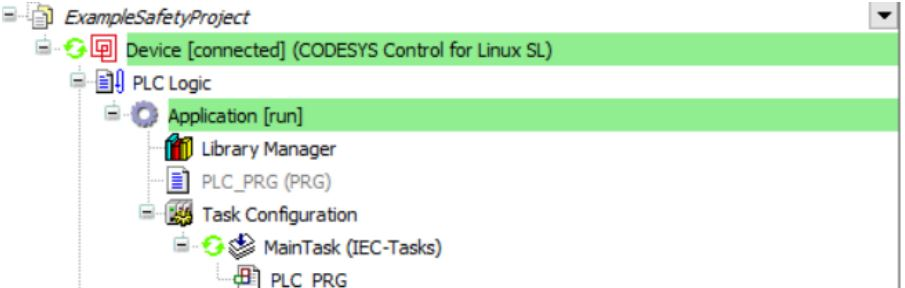
\includegraphics[width=1\textwidth]{e7.JPG}
\end{figure}
As previously described, the Safe Control log can be checked to confirm the connection to the timer.

% Selecting the SafetyApp as the active application
The \texttt{Safe Control SafetyApp} can then be selected as the active application. Via the communication dialog of the device, you can log in to the safety controller.
\begin{figure}[H]
	\centering
	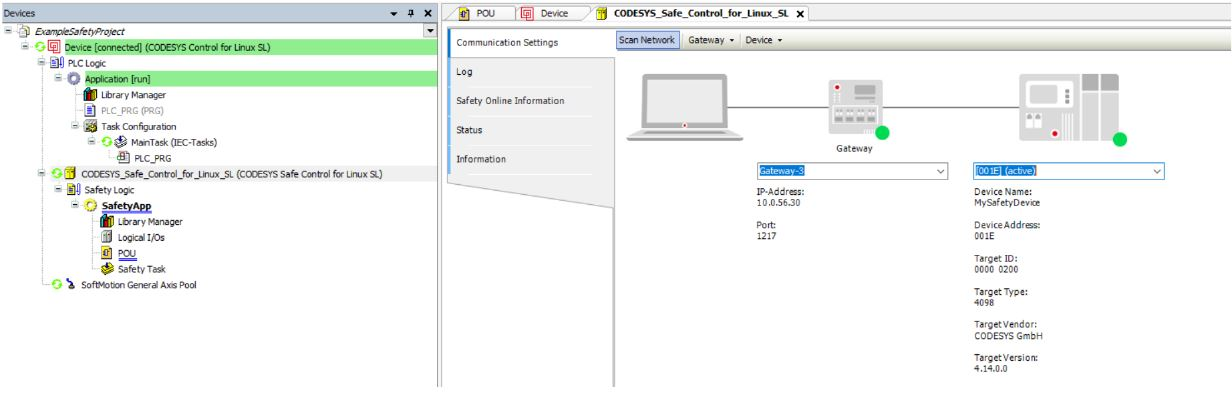
\includegraphics[width=1\textwidth]{e8.JPG}
\end{figure}
% Handling the download type prompt
After logging in, a yellow dialog window will prompt for the type of download.
\begin{figure}[H]
	\centering
	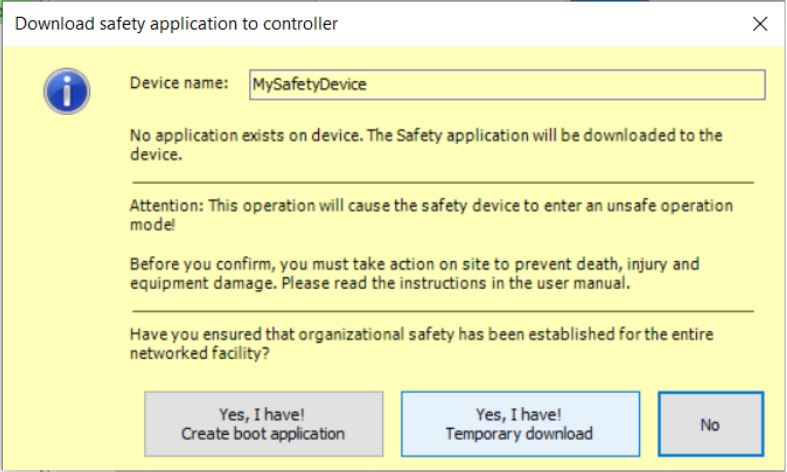
\includegraphics[width=0.7\textwidth]{e9.JPG}
\end{figure}
For a brief test of the counter, a temporary download can be performed. A window will then open, requesting a password.

% Handling the password prompt for the download
Since no password has been defined on the controller yet, the field can be left empty and confirmed by clicking \texttt{OK}.
\begin{figure}[H]
	\centering
	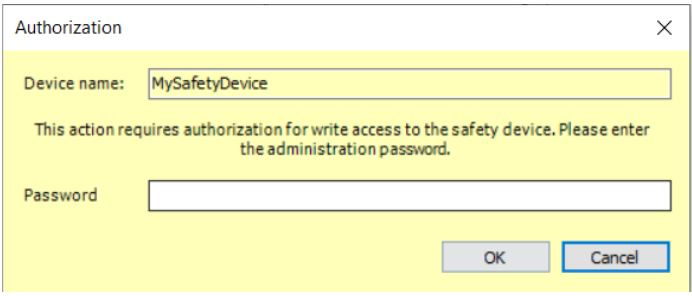
\includegraphics[width=0.7\textwidth]{e10.JPG}
\end{figure}
% Running and verifying the application
The application is then downloaded and in the \texttt{Stop} state. After starting the application, the \texttt{counter} variable in the POU should cyclically increment. 
\begin{figure}[H]
	\centering
	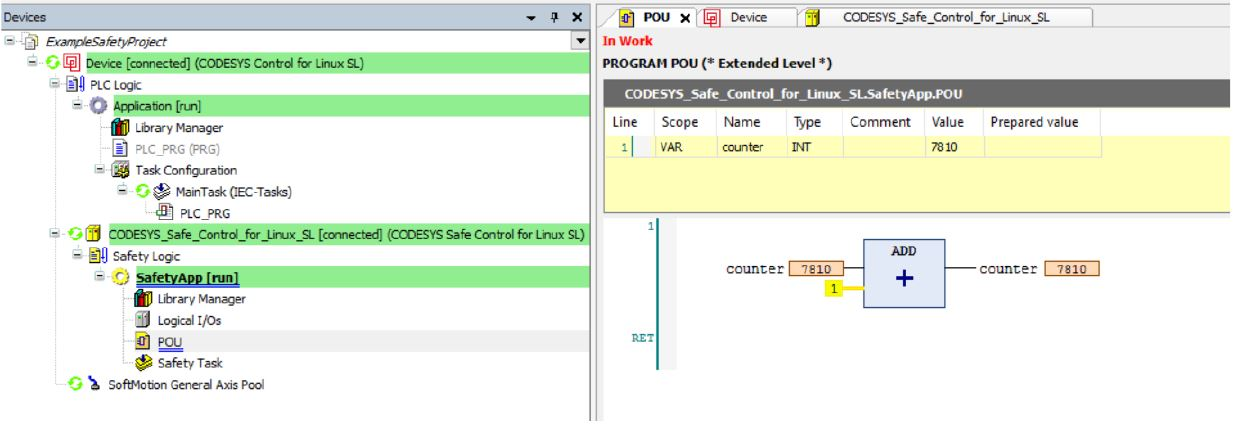
\includegraphics[width=1\textwidth]{e11.JPG}
\end{figure}
During a normal download (DL), the program still runs in the unsafe state (DL).
\begin{figure}[H]
	\centering
	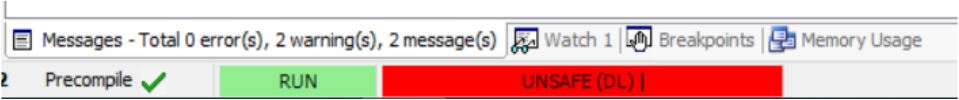
\includegraphics[width=1\textwidth]{e13.JPG}
\end{figure}
% Creating a boot application for safe operation
To run the program in a safe state, a boot application must be created on the safety controller. Creating the boot application requires logging out of the safety controller, which unloads the download.

% Selecting and sealing the boot application
\begin{figure}[H]
	\centering
	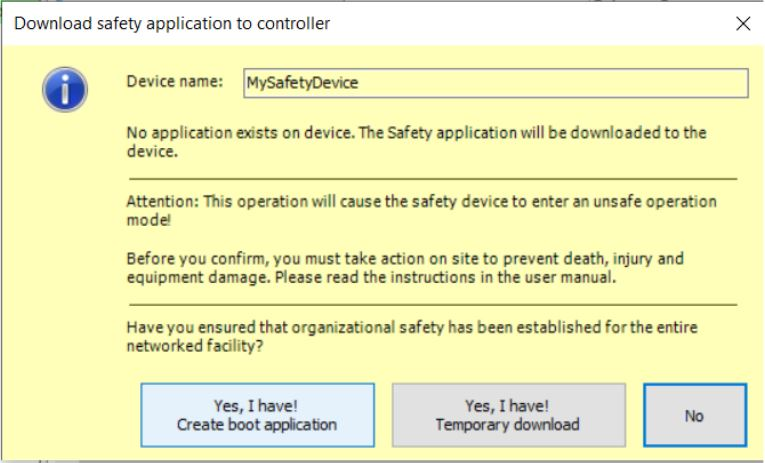
\includegraphics[width=0.8\textwidth]{e14.JPG}
\end{figure}
The boot application is then selected. You will be prompted to confirm whether you want to create the boot application, which must be confirmed with \texttt{Yes}. 
\begin{figure}[H]
	\centering
	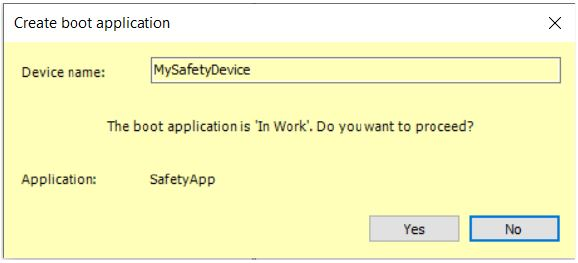
\includegraphics[width=0.8\textwidth]{e15.JPG}
\end{figure}
Subsequently, you will receive confirmation that the boot application has been created on the device. The application is now in the \texttt{Stop} state again.
\begin{figure}[H]
	\centering
	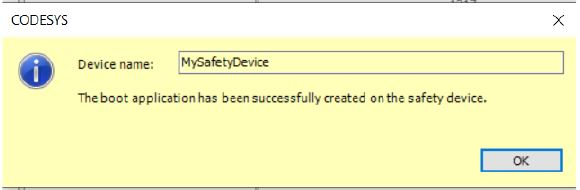
\includegraphics[width=1\textwidth]{e16.JPG}
\end{figure}
 After starting the application, it remains in the unsafe state but with a boot application
\begin{figure}[H]
	\centering
	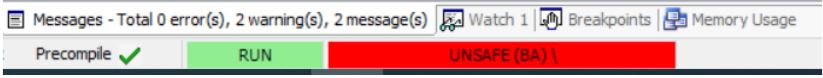
\includegraphics[width=1\textwidth]{e17.JPG}
\end{figure}

To enter the safe state during the boot application, a logout is necessary along with the confirmation of the restart of the boot application.
\begin{figure}[H]
	\centering
	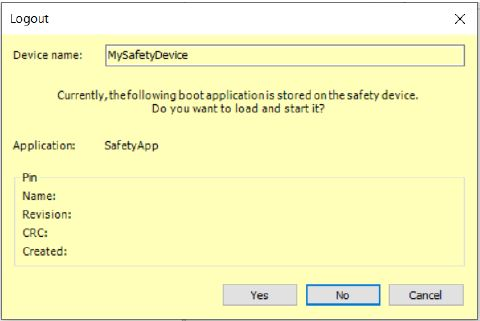
\includegraphics[width=0.8\textwidth]{e18.JPG}
\end{figure}
\begin{figure}[H]
	\centering
	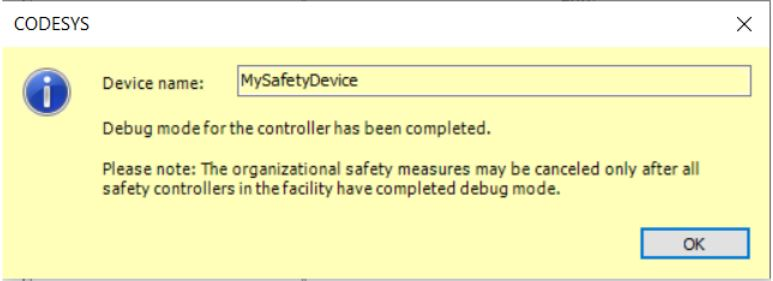
\includegraphics[width=0.8\textwidth]{e19.JPG}
\end{figure}
Now the application has been restarted.
\begin{figure}[H]
	\centering
	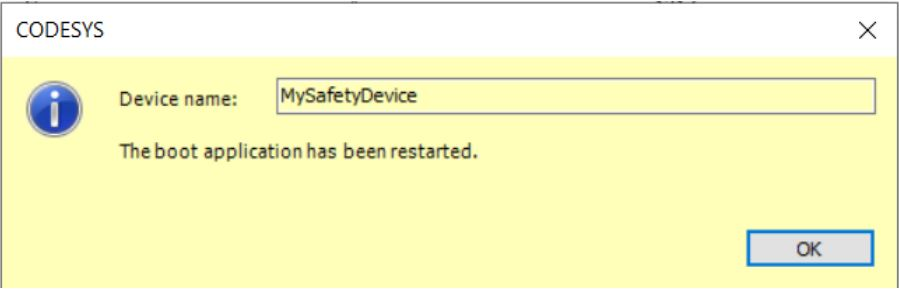
\includegraphics[width=0.8\textwidth]{e19e20.JPG}
\end{figure}
To view the status of the boot app, the Safety Online Information dialog from the Safe Control can be accessed.

\begin{figure}[H]
	\centering
	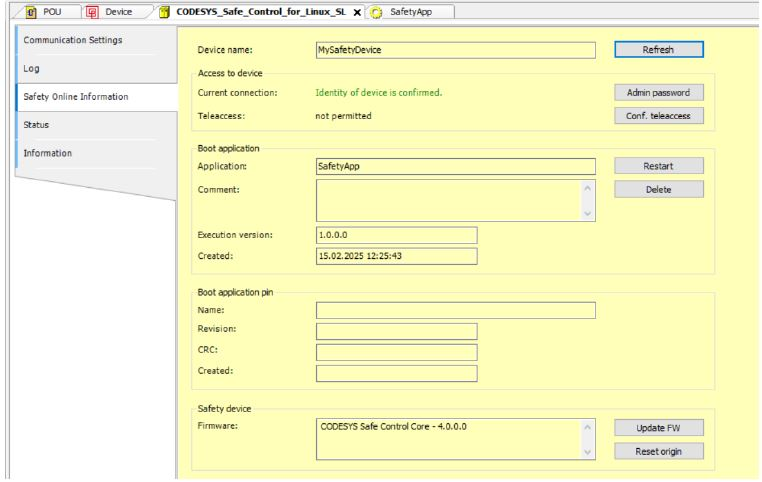
\includegraphics[width=0.8\textwidth]{e21.JPG}
\end{figure}
After logging in again to the safety controller, a confirmation to start the boot app is requested in the log messages from the Safety Runtime.
\begin{figure}[H]
	\centering
	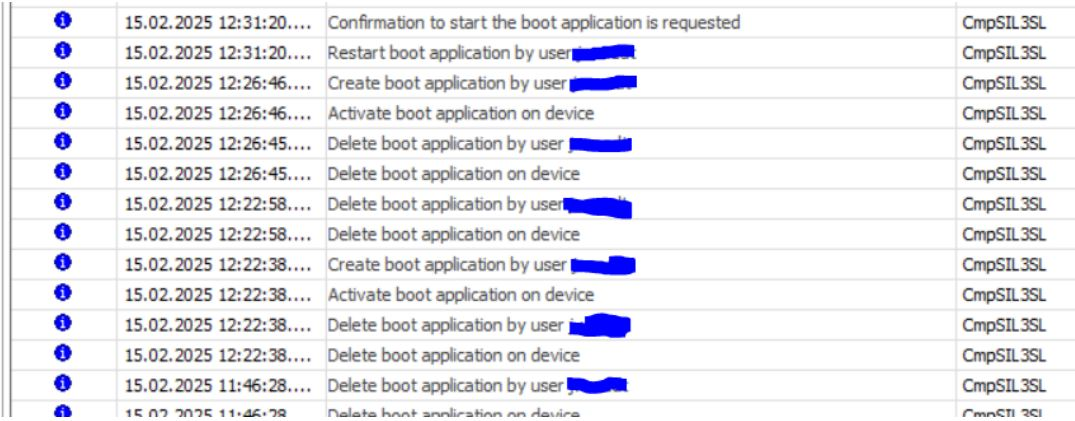
\includegraphics[width=0.8\textwidth]{e22.JPG}
\end{figure}
The application is now in the safe state but has not yet started.
\begin{figure}[H]
	\centering
	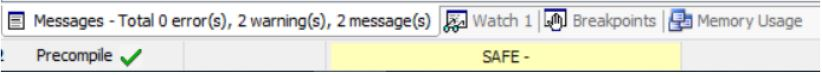
\includegraphics[width=1\textwidth]{e23.JPG}
\end{figure}
The start of the boot app is performed via the non-safe standard controller. For this purpose, a program was created that implements the \texttt{SafeControl.StartBootApp} FB.

\begin{figure}[H]
	\centering
	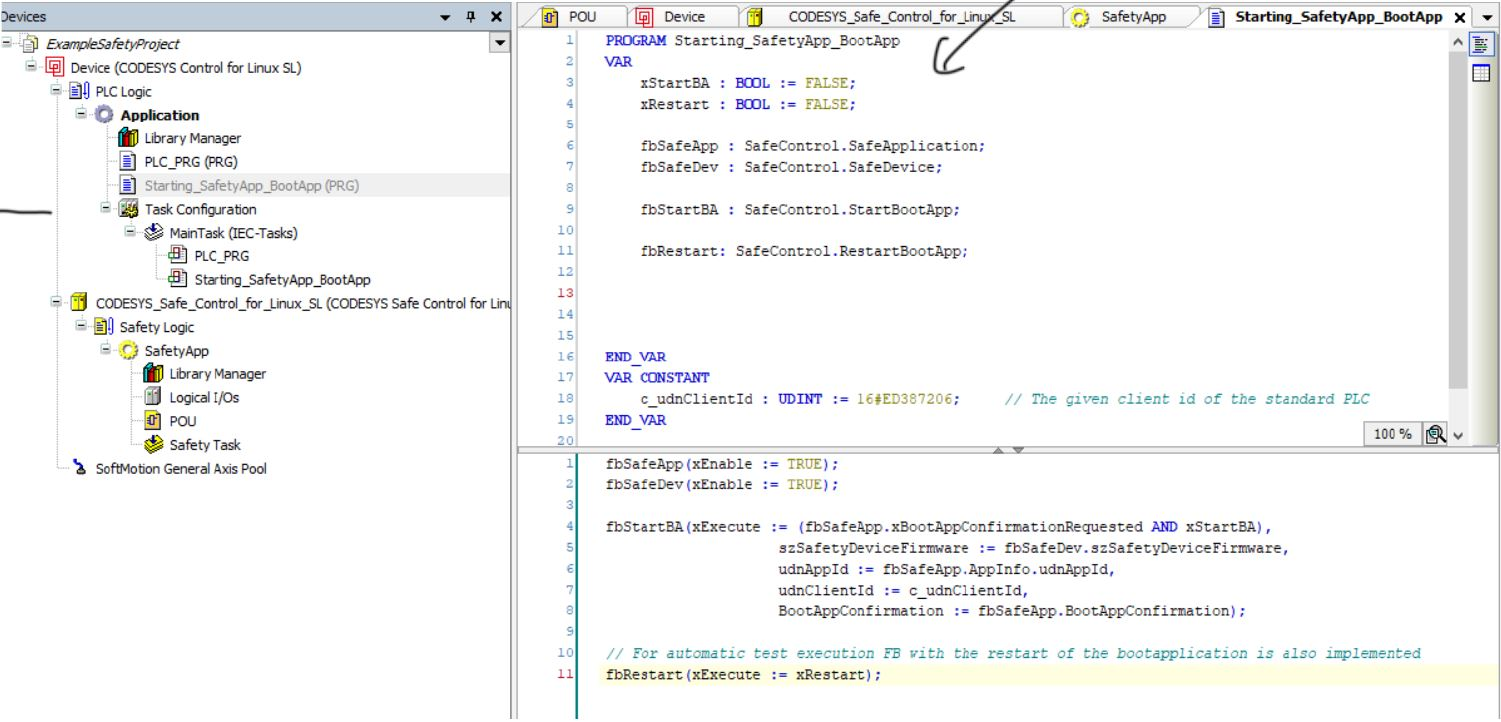
\includegraphics[width=1\textwidth]{e24.JPG}
\end{figure}
Code:
\begin{verbatim}
	PROGRAM Starting_SafetyApp_BootApp
	VAR
	xStartBA : BOOL := FALSE;
	xRestart : BOOL := FALSE;
	
	fbSafeApp  : SafeControl.SafeApplication;
	fbSafeDev  : SafeControl.SafeDevice;
	
	fbStartBA  : SafeControl.StartBootApp;
	fbRestart  : SafeControl.RestartBootApp;
	END_VAR
	
	------------------------------------------------------------
	
	VAR CONSTANT
	c_udnClientId : UDINT := 16#ED387206;   // The given client id of the standard PLC
	END_VAR
	
	fbSafeApp(xEnable := TRUE);
	fbSafeDev(xEnable := TRUE);
	
	fbStartBA(xExecute := (fbSafeApp.xBootAppConfirmationRequested AND xStartBA),
	szSafetyDeviceFirmware := fbSafeDev.szSafetyDeviceFirmware,
	udnAppId := fbSafeApp.AppInfo.udnAppId,
	udnClientId := c_udnClientId,
	BootAppConfirmation := fbSafeApp.BootAppConfirmation);
	
	// For automatic test execution FB with the restart of the bootapplication is also implemented
	fbRestart(xExecute := xRestart);
\end{verbatim}

\newpage
With the variable \texttt{xStartBA}, the boot application can be manually activated.
\begin{figure}[H]
	\centering
	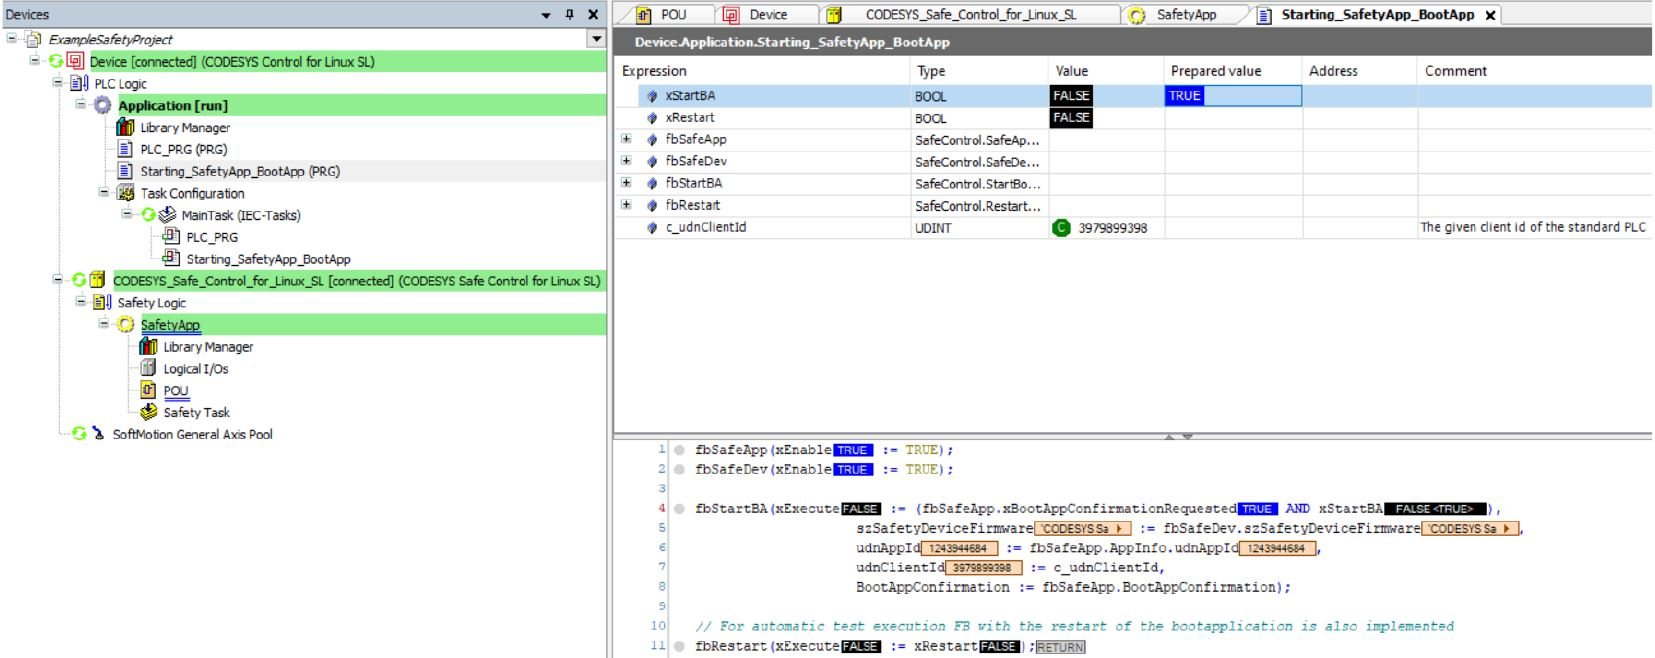
\includegraphics[width=1\textwidth]{e25.JPG}
\end{figure}
Subsequently, the Safe Control is started and is in the safe state (BA).
\begin{figure}[H]
	\centering
	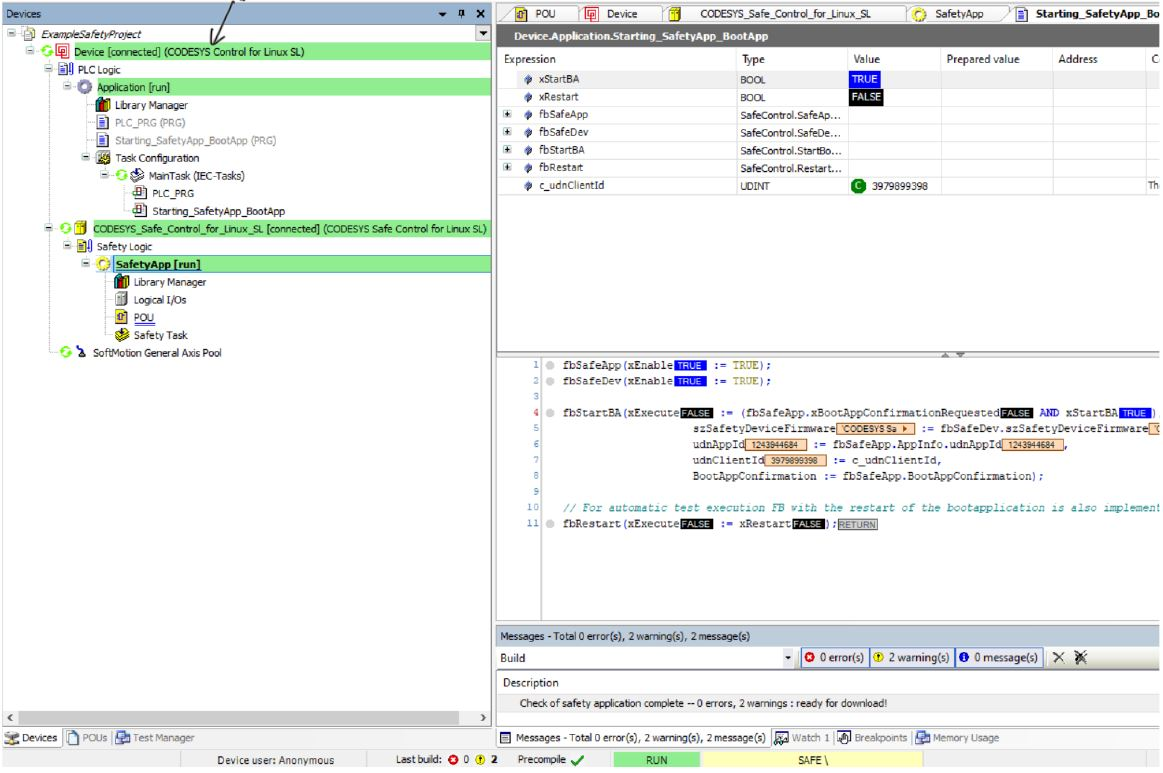
\includegraphics[width=1\textwidth]{e26.JPG}
\end{figure}


\subsection{Location of the Configuration File and Client ID for Safety Runtime}

For the boot application confirmation, a \textbf{Client ID} is required. The configuration file of the Safe Control runtime system contains a default Client ID.

It is also possible to define custom Client IDs individually in this configuration file.

For the package-based Safe Control system, the configuration file can be found in the following directory on the Linux host:

\begin{verbatim}
	/etc/codesyssafecontrol
\end{verbatim}

\begin{figure}[H]
	\centering
	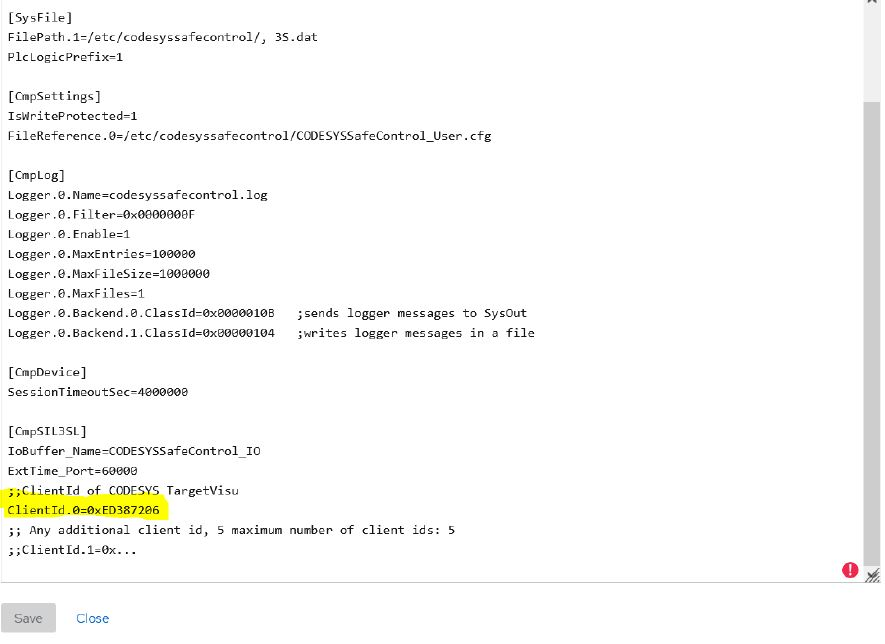
\includegraphics[width=1\textwidth]{16.JPG}
\end{figure}

The log files for the Safe Control runtime system are stored in:

\begin{verbatim}
	/var/opt/codesyssafecontrol
\end{verbatim}

\subsection{Renaming the Safe Control Device}

Renaming the safety controller is possible via the communication settings:

\texttt{Device → Active Device → Rename}
\begin{figure}[H]
	\centering
	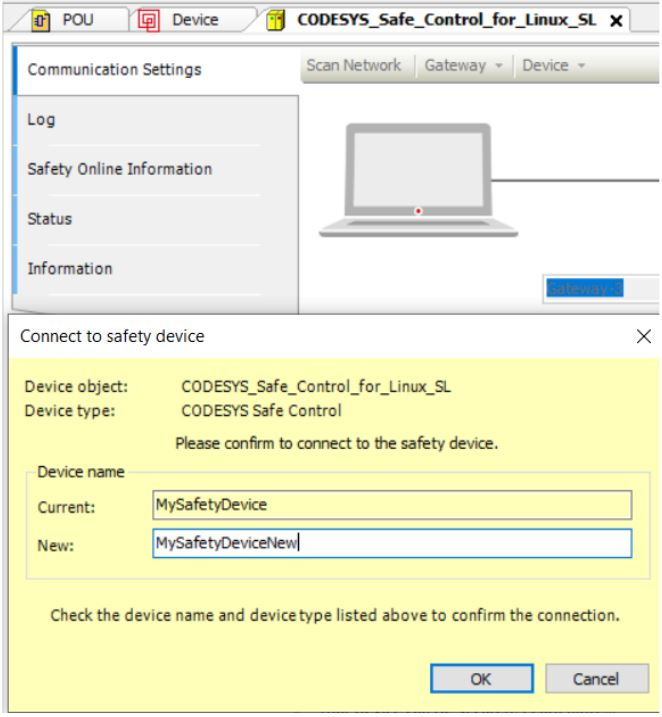
\includegraphics[width=0.5\textwidth]{17.JPG}
\end{figure}


\section{Logical Devices}

\subsection{Data Exchange Between Safety and Standard Controller}

To set up data exchange between the safety and standard controller, follow these steps:

\begin{enumerate}
	\item In the safety controller:
	\begin{itemize}
		\item Navigate to \texttt{<Safety-Device> → Safety Logic → SafetyApp → Logical I/Os}.
		\item Open the context menu and select the command \textbf{Add Logical Device}.
		\item In the dialog, select an object from the \textbf{Logical Exchange Devices} node.
	\end{itemize}
	\begin{figure}[H]
		\centering
		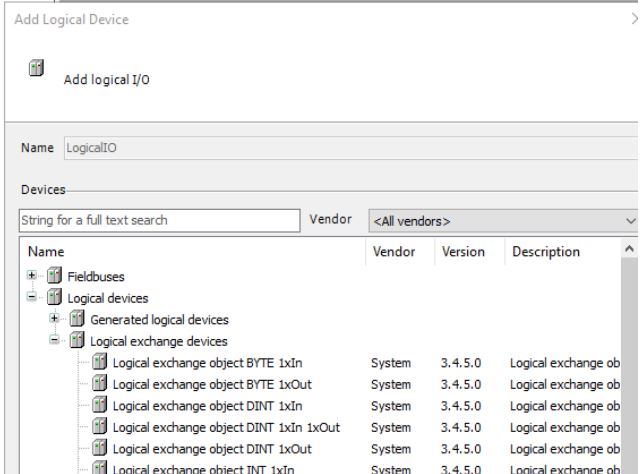
\includegraphics[width=0.6\textwidth]{18.JPG}
	\end{figure}
	
	\item In the standard controller:
	\begin{itemize}
		\item Navigate to \texttt{<Standard-Device> → PLC Logic → Application}.
		\item Open the context menu and select \textbf{Add Object → Logical Exchange GVL}.
		\item Give the object an appropriate name and add it to the project tree.
	\end{itemize}
	\begin{figure}[H]
		\centering
		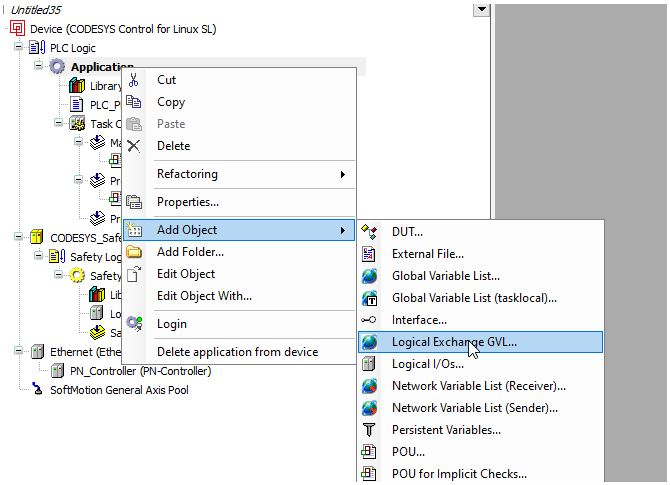
\includegraphics[width=0.7\textwidth]{19.JPG}
	\end{figure}
	
	\item In the editor:
	\begin{itemize}
		\item Link the logical exchange device with the GVL (Global Variable List).
	\end{itemize}
\end{enumerate}

\subsection{Exchange Fieldbus with Safe I/Os}
The exchange of I/O data is also performed via logical devices. If the assignment is unambiguous (e.g., only one safety controller in the project tree), inserting the physical device automatically adds and links the logical device under \texttt{Logical I/Os} in the Safety Application.

The linkage is displayed:
\begin{itemize}
	\item In the project tree, behind the name of both the physical and logical device as \texttt{[$\rightarrow$]} or \texttt{[$\leftarrow$]}.
	\begin{figure}[H]
		\centering
		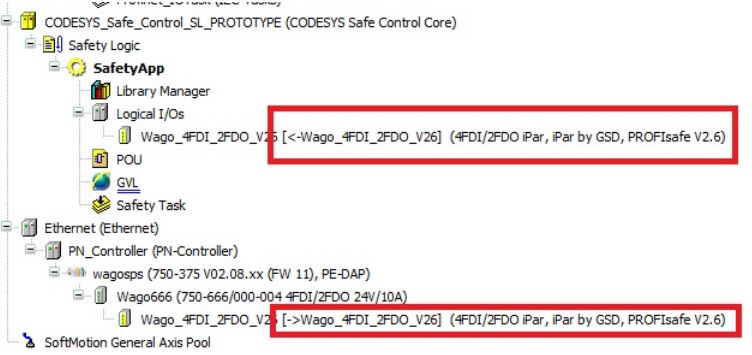
\includegraphics[width=0.8\textwidth]{21.JPG}
	\end{figure}
	\item In the Mapping Editor of the physical device.
	\begin{figure}[H]
		\centering
		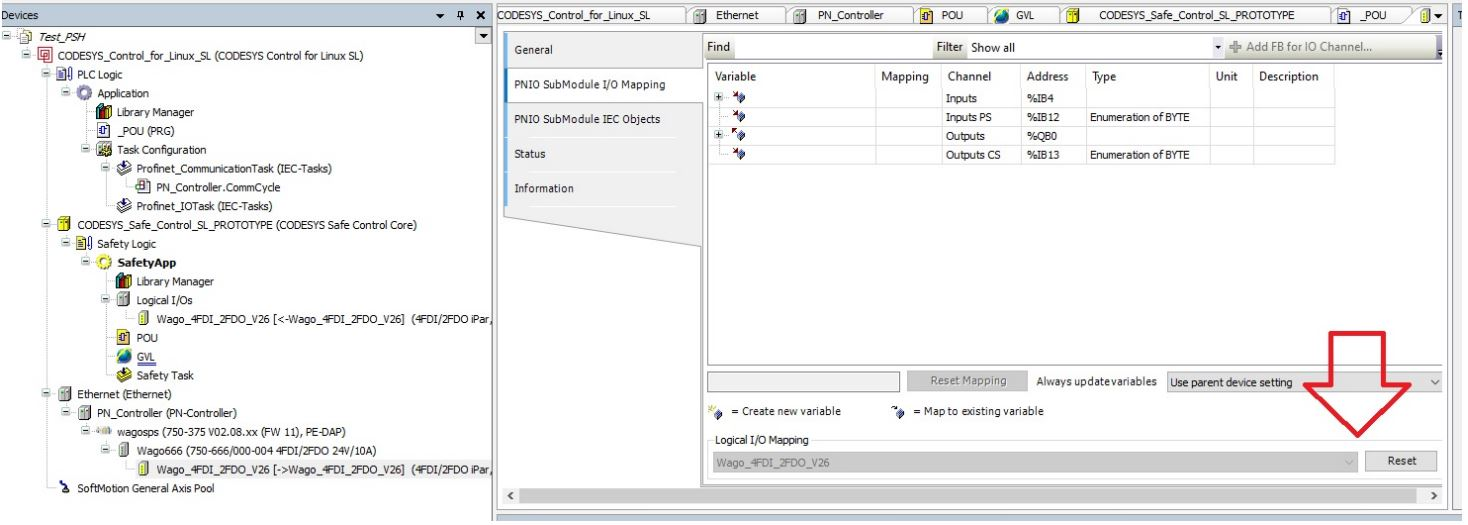
\includegraphics[width=1\textwidth]{22.JPG}
	\end{figure}
\end{itemize}

In the Mapping Editor of the physical device, the linkage can be reset or re-established.

\textbf{Product Marketing}: Set up Debian + vPLC + vSafePLC from scratch. \\
\textbf{CODESYS Project}: For using CODESYS Safe Control – 33.

For the inserted logical device, a global function block (FB) instance is created in the Safety Application with the variable name and type corresponding to the logical device. The FB instance is uniquely defined in the Safety Mapping Editor of the logical device.
\begin{figure}[H]
	\centering
	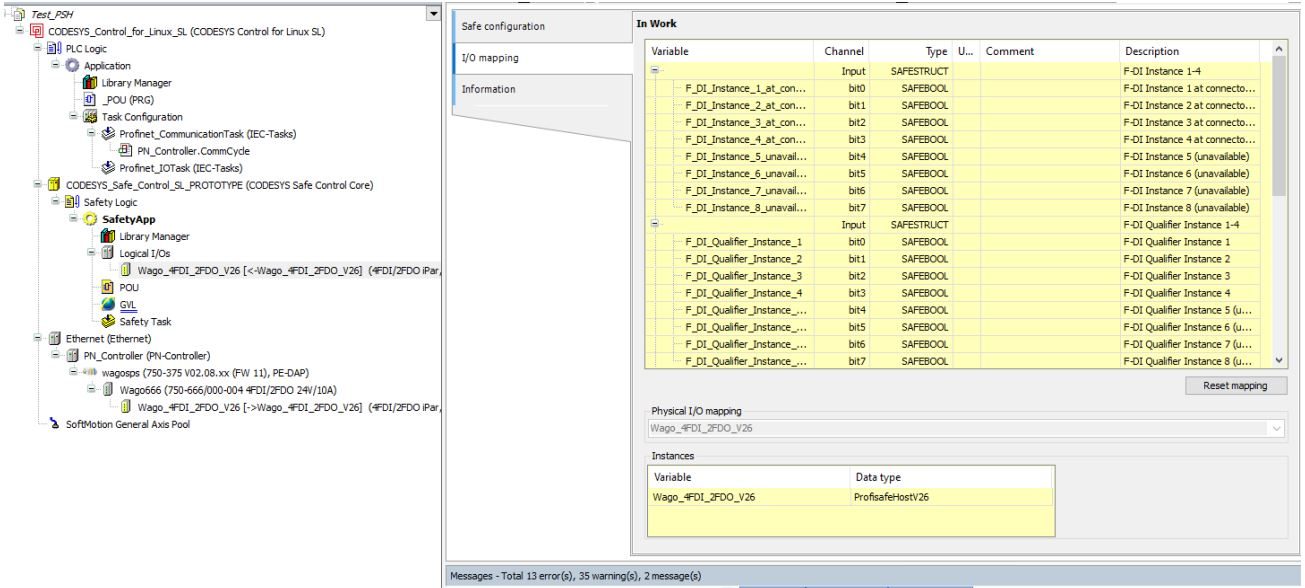
\includegraphics[width=1\textwidth]{23.JPG}
\end{figure}

\textbf{Note}: When inserting, the logical device name may start with an underscore (\texttt{\_}). However, the FB instance starts with \texttt{x\_} (starting from SafetyVersion 4.2; previously, this caused a build error).

Fieldbuses supported for SIL3 with safe I/Os:
\begin{itemize}
	\item PROFInet with PROFIsafe V2.4
	\item PROFInet with PROFIsafe V2.6 (only for Safe Control Core)
	\item EtherCAT with FSoE (planned for Safe Control Core)
\end{itemize}

\subsection{PROFIsafe}
Two versions are available: PROFIsafe V2.4 and V2.6. New F-Device devices must only support V2.6. The physical device defines the version, which is not switchable.

\subsection{Safety Application}
A list of objects.
\begin{figure}[H]
	\centering
	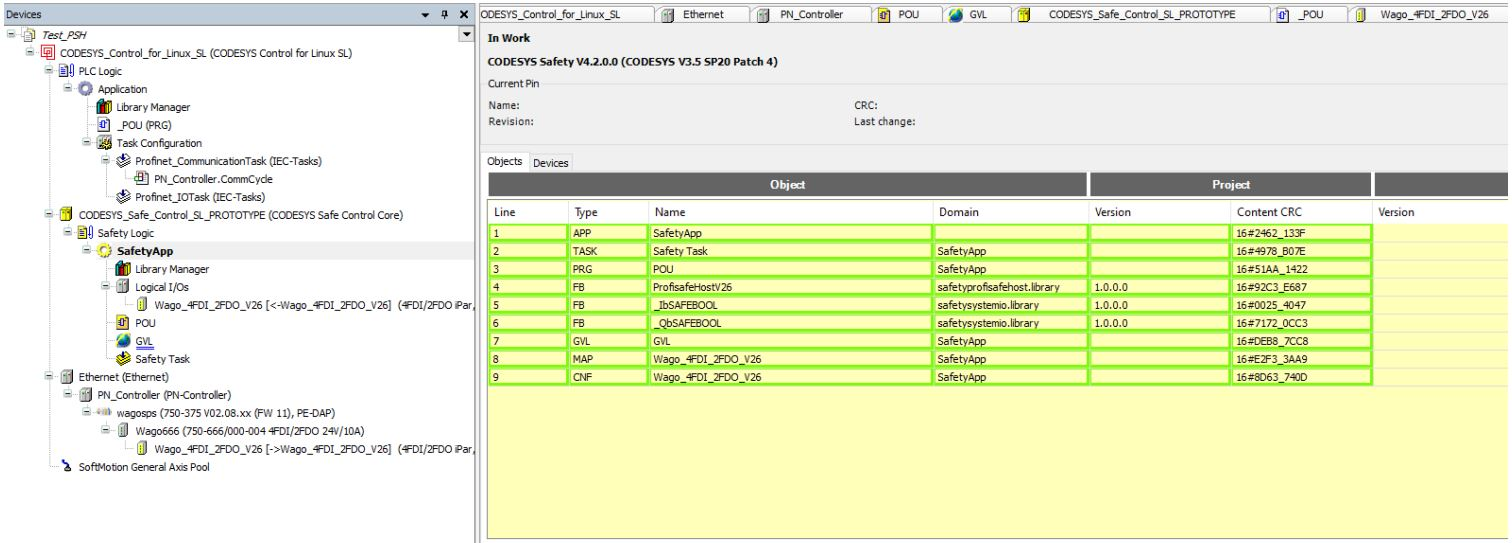
\includegraphics[width=1\textwidth]{24.JPG}
\end{figure}
Each object corresponds to a ``yellow'' editor. Every object editor stores the data in a 1:1 ``Interpreter'' format, which is loaded into the Safety Runtime during download. Additionally, the Safety Runtime expects information from the Safety Checker, which is executed during the ``Build'' or before the ``Login with Download''.

\subsection{Global Variable List (GVL)}
\textbf{Note}: No namespace is used for the GVL. GVL variables are accessed via \texttt{VAR EXTERNAL}. This is not an issue since variable names in a Safety Application must be unique.

\subsection{IO Mapping}
Defines the variables mapped into the Safety Application. Variable definitions are implicitly of type Global and are used in the Safety Application's POUs with \texttt{VAR\_EXTERNAL}. 

In the Mapping Editor, the linkage to the physical device and the global function block (FB) instance of the corresponding IO stack is displayed.

\textbf{Note}: In the Mapping Editor, a byte must be defined either as a single byte or as individual bits; mixing both is not allowed.

\subsection{IO Configuration (F-Parameter)}
Settings corresponding to the assigned physical safe I/O device. For PROFIsafe or FSoE F-devices, the F-Destination Address is set via DIP switches on the IO or assigned using a device-manufacturer-specific tool.

\subsection{POU, FB}
Two different object types:

\textbf{Product Marketing}: Set up Debian + vPLC + vSafePLC from scratch. \\
\textbf{CODESYS Project}: For using CODESYS Safe Control – 35.

\begin{itemize}
	\item \textbf{Basic}: Only FBs with combinatorial logic of boolean operations using \texttt{AND} or \texttt{OR}. No \texttt{NOT}!
	\item \textbf{Extended}: Full range of supported operators (see Toolbox).
\end{itemize}

\textbf{Note}: Safety programming strictly distinguishes between logical and numerical data types. Numerical operations cannot be performed on logical data types, and logical operations cannot be performed on numerical data types.

\begin{itemize}
	\item \textbf{Logical Data Types}: \texttt{BOOL}, \texttt{BYTE}, \texttt{WORD}, \texttt{DWORD}, etc., with operations \texttt{AND}, \texttt{OR}, \texttt{NOT}.
	\item \textbf{Numerical Data Types}: \texttt{INT}, \texttt{UINT}, \texttt{DINT}, etc., with operations \texttt{ADD}, \texttt{SUB}, \texttt{DIV}, \texttt{MUL}, \texttt{LE}, \texttt{GT}, etc.
\end{itemize}

Structures, arrays, enums, and pointers are not supported!

\subsection{Safety Task}
Only one cyclic task with a specified cycle time, default 10 ms. The selected programs in the list are executed in the order of the task list. The execution order can be controlled using \texttt{Up}, \texttt{Down}, or selection (\texttt{All}, \texttt{None}).

\section{Diagnosis}
\subsection{Exchange Between Safety and Standard}
Configuration ID via the module list of exchanged devices, \texttt{IoDrvSafetySP}. The device tree indicates whether the ID matches at the Safety Controller.

\textbf{Note}: Changes to the PROFIsafe configuration, e.g., \texttt{F\_WD\_Time}, also require a download of the Standard. The CRC of the F-Parameters is part of the Configuration ID, and a mismatch is displayed to the user in the project tree.

\subsection{IO-Stack Instance}
See online help: \url{https://content.helpme-codesys.com/en/CODESYS\%20Safety\%20Extension/sil3_field_buses.html}.

Meaning of the FB output Diagnosis:
\begin{itemize}
	\item \texttt{0x8xxx}: OK, with \texttt{xxx} indicating status.
	\item \texttt{0xC0xx}: Initialization error \texttt{XX}, usually with a logbook entry, application terminated.
	\item \texttt{0xC1xx}: Self-detected error \texttt{XX}.
	\item \texttt{0xC2xx}: Error \texttt{XX} detected by the F-Device.
\end{itemize}

\subsubsection{PROFIsafe}
Different behavior regarding FB Diagnosis Output:
\begin{itemize}
	\item \textbf{V2.4}: Diagnosis word is overwritten by higher-priority diagnosis, priority from \texttt{16\#C0xx} to \texttt{16\#C2xx}.
	\item \textbf{V2.6}: The first detected error remains as the diagnosis word at the FB output until acknowledged.
\end{itemize}

\textbf{Product Marketing}: Set up Debian + vPLC + vSafePLC from scratch. \\
\textbf{CODESYS Project}: For using CODESYS Safe Control – 36.

\textbf{Note}: The F-Host recognizes only two errors: Timeout or CRC error. The CRC error includes all possible variants of initialization and communication errors.

PROFIsafe Diagnosis on Standard (only Safe Control Core: F-Host Outputs are transferred to Standard). Example access:

\textbf{Declaration}:
\begin{lstlisting}
uiID: UDINT;
FHostState: ProfinetCommon.F_HostStatus;
\end{lstlisting}

\textbf{Implementation}:
\begin{lstlisting}
(* Next code line requires lib IoDrvProfinetBase! *)
uiID := IoDrvProfinetBase.GetID(Wago666);
ProfiNetCommon.GetFHostStatus(ID := uiID, F_Status := FHostState);
\end{lstlisting}

\section{Download - Boot Application}
\textbf{Note}: Handling of Download and Boot Application differs from Standard. With a logout, a running application is unloaded and no longer executed. If a Boot Application exists on the controller, it may or may not be started.

For Safety Controllers, the Login dialog requires a decision on whether to perform only a Download or a Download with Boot Application creation. Download with Boot Application combines two commands (Login and Create Boot Application), which can generally be executed independently.

A Download with Boot Application takes longer since the source code is loaded to the controller twice: once for the Download and once for the Boot Application. Therefore, it is recommended to perform a Download first and create a Boot Application only when the application is stable.

\subsection{Start of the Boot Application for SafeControl Core}
The start of the Boot Application differs between SIL3 OEM controllers and Safe Control Core. For Safe Control Core, the user must confirm the start of the Boot Application. This is supported by the CODESYS Safe Control Lib (see Diagnosis on Standard).

Starting from Safety Extension 4.3.0.0, the status is displayed in the project tree and the active application status (see screenshot). For Safety Extension versions earlier than 4.3.0.0, no display is available in either the tree or the status, and both fields are empty.

\begin{figure}[H]
	\centering
	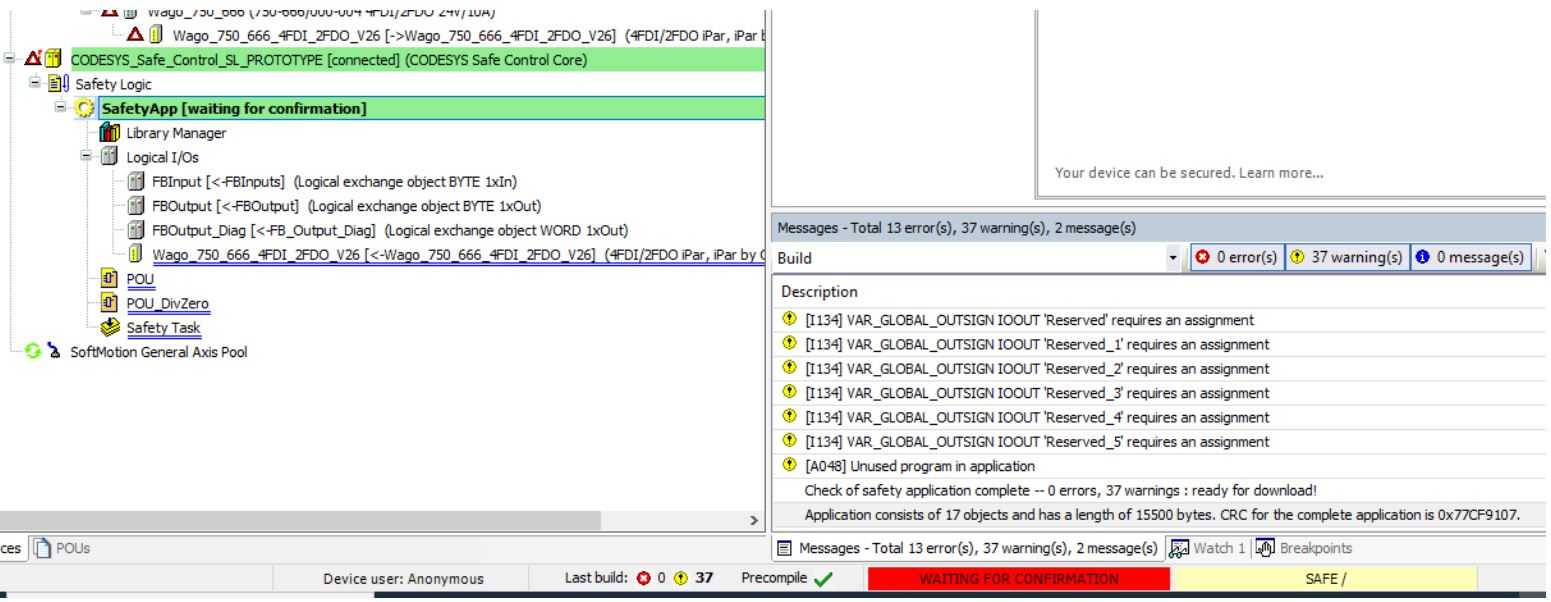
\includegraphics[width=1\textwidth]{25.JPG}
\end{figure}

\section{Diagnosis on Standard}
The CODESYS Safe Control Service Package includes the \texttt{CODESYS Safe Control} library, providing the following function blocks (FBs):

\begin{figure}[H]
	\centering
	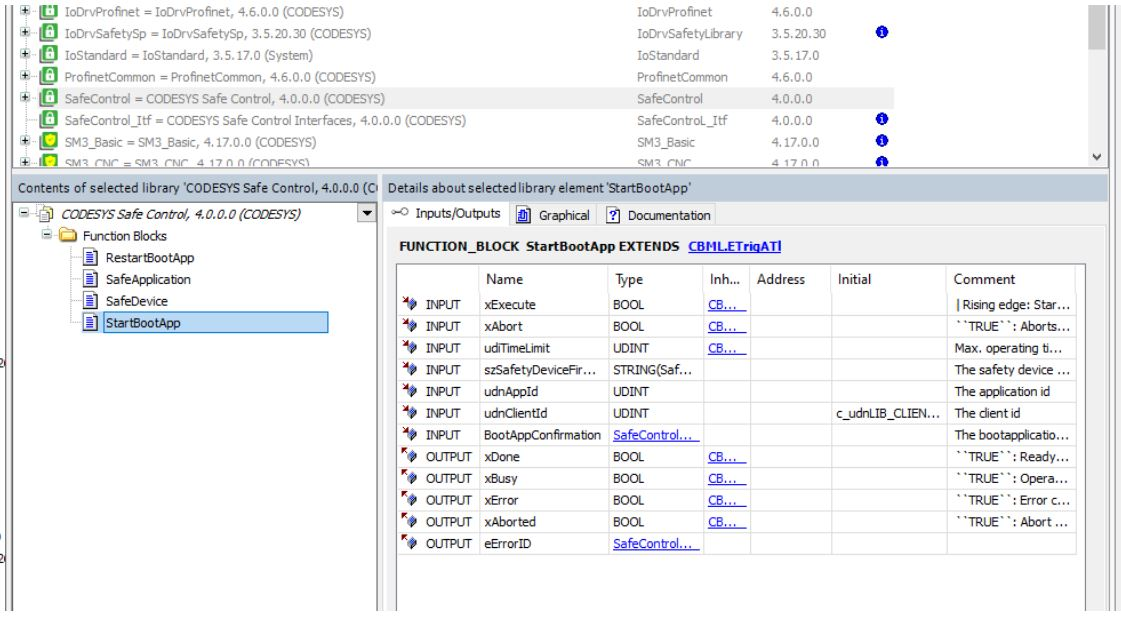
\includegraphics[width=1\textwidth]{26.JPG}
\end{figure}

\begin{itemize}
	\item \textbf{FB SafeDevice}: Provides information and diagnostics about the device. \textbf{Note}: Information regarding external timers is currently not meaningfully usable (see Jira SIL3SL-725).
	\item \textbf{FB SafeApplication}: Provides information about the loaded application or the start of the Boot Application.
	\item \textbf{FB StartBootApp}: FB for confirming the start of the loaded Boot Application. Starting from Safety Extension 4.3.0.0, this additional state is displayed in the project tree and in the status of the active application. For versions earlier than 4.2.0.0, no application status is displayed.
\end{itemize}

To start the Boot Application, the current value of the FB output \texttt{SafeApplication.BootAppConfirmation} must be specified, along with a Client ID defined in the runtime's CFG file. The default for the Standard Application is \texttt{16\#ED387206}.

\textbf{Product Marketing}: Set up Debian + vPLC + vSafePLC from scratch. \\
\textbf{CODESYS Project}: For using CODESYS Safe Control – 38.

\textbf{ApplicationId}: Starting from version 4.3.0.0, available via the command \texttt{Build $\rightarrow$ Show Details about Active Safety Application}.
\begin{figure}[H]
	\centering
	\includegraphics[width=0.8\textwidth]{27.JPG}
\end{figure}

\textbf{Example Implementation for Boot Application Start Confirmation}:

\textbf{Declaration}:
\begin{lstlisting}
PROGRAM StartSafetyBA
VAR
xStartBA : BOOL := FALSE;
xRestart : BOOL := FALSE;

fbSafeApp : SafeControl.SafeApplication;
fbSafeDev : SafeControl.SafeDevice;

fbStartBA : SafeControl.StartBootApp;

fbRestart: SafeControl.RestartBootApp;

END_VAR
VAR CONSTANT
c_udnClientId : UDINT := 16#ED387206;     // The given client id of PLC
END_VAR
\end{lstlisting}

\textbf{Implementation}:
\begin{lstlisting}
fbSafeApp(xEnable := TRUE);
fbSafeDev(xEnable := TRUE);
fbStartBA(xExecute := (fbSafeApp.xBootAppConfirmationRequested AND xStartBA), 
szSafetyDeviceFirmware := fbSafeDev.szSafetyDeviceFirmware, 
udnAppId := fbSafeApp.AppInfo.udnAppId, 
udnClientId := c_udnClientId,
BootAppConfirmation := fbSafeApp.BootAppConfirmation);
// For automatic test execution FB with the restart of the bootapplication is also implemented
fbRestart(xExecute := xRestart);
\end{lstlisting}



\section{Debugging}
Only online commands are supported: \texttt{Start}, \texttt{Stop}, \texttt{Write}, and \texttt{Force}. Forcing is limited to a maximum of 20 entries.

\section{Device Editors}
\begin{itemize}
	\item Communication
	\item Safety Online Information
	\item Status
	\item Information
\end{itemize}

\section{Additional Restrictions}
\textbf{Lib-Manager}: Users cannot develop libraries; this is not supported. Currently, only libraries with external FBs are available.

\subsection{Further Links}
\begin{itemize}
	\item Online Help for Virtual Safe Control: \url{https://content.helpme-codesys.com/de/CODESYS%20Control/_rtsl_scenario_safe_house.html}
	\item Docker Installation: \url{https://docs.docker.com/engine/install/debian/}
\end{itemize}

\newpage
\section{Use Case: Virtual Safe Emergency Stop}

\subsection{Opening the Project}

To begin, open the project \textbf{vSafeTest\_sim}, located in the appendix.

\begin{figure}[H]
	\centering
	\includegraphics[width=0.8\textwidth]{c1.JPG}
\end{figure}

After a brief loading period, a project environment popup will appear. Click \textbf{OK} in the bottom-right corner to continue.

Once the project has fully loaded, navigate to the \textbf{Application} section under \textbf{Device}, and click \textbf{Login} to establish a connection with the device.

\begin{figure}[H]
	\centering
	\includegraphics[width=0.8\textwidth]{c2.JPG}
\end{figure}

The \textbf{VGateway} should already be pre-selected. Use the same login credentials as previously used. For detailed information on logging into the Safe POU, refer to Section~\ref{sec:safe-pou-changes}.

Next, log into the Safe Control by right-clicking on \textbf{SafetyApp} and selecting \textbf{Login}. This action establishes the connection to both the standard and safe systems.

Once the connection is successful, both devices will show green status indicators. Additionally, the central status bar will display \textbf{RUN} in green and \textbf{SAFE} in yellow. The device icons on the right-hand side of the screen will also appear green.

\begin{figure}[H]
	\centering
	\includegraphics[width=\textwidth]{c3.PNG}
\end{figure}

\subsection{Handling Version Compatibility Issues}

If you encounter version compatibility issues, right-click on the affected device and select \textbf{Update Device}. A popup window will appear, allowing you to choose the correct version. For this project, select \textbf{Linux SL 4.15.0.0}.

\begin{figure}[H]
	\centering
	\includegraphics[width=0.4\textwidth]{c4.jpg}
\end{figure}

To update the Safe Control version, select \textbf{CODESYS Safe Control}, click \textbf{Update Device}, and choose the appropriate version number—again, \textbf{4.15.0.0}.

\begin{figure}[H]
	\centering
	\includegraphics[width=0.4\textwidth]{c5.jpg}
\end{figure}

\subsection{Testing the Emergency Stop}

To test the emergency stop (\textit{Not-Aus}), open the \textbf{Visualization} view. Toggle the switch labeled \textbf{Logical GVL Safe Out} to simulate an emergency stop. When the lever is flipped, the LED on the \textbf{EStop} indicator should turn on.

\begin{figure}[H]
	\centering
	\begin{minipage}{0.4\textwidth}
		\centering
		\includegraphics[width=\textwidth]{c6.jpg}
		\caption*{Flip the lever}
	\end{minipage}
	\hspace{0.02\textwidth}
	{\Huge$\Rightarrow$}
	\hspace{0.02\textwidth}
	\begin{minipage}{0.4\textwidth}
		\centering
		\includegraphics[width=\textwidth]{c7.jpg}
		\caption*{EStop LED lights up}
	\end{minipage}
\end{figure}

This confirms that the emergency stop simulation was triggered correctly and that both the visual feedback and system response function as intended. With this, the setup and validation of the virtual safety mechanism are complete.




\end{document}
